\documentclass[review]{siamart220329}

% Package import
\usepackage[utf8]{inputenc}
\usepackage{graphicx,subfig}
\usepackage{amstext,amsmath,amssymb,bm,bbm,mathtools}
\usepackage{algorithmic}
\usepackage[export]{adjustbox}
\usepackage{array,multirow}
\usepackage{amsmath}
\usepackage{amssymb}
\usepackage{changes}

% Custom Math Definitions
\DeclareMathOperator*{\argmin}{arg\,min}
\DeclarePairedDelimiter\norm{\lVert}{\rVert}%
\DeclarePairedDelimiter\abs{\lvert}{\rvert}%

% Custom Commands
\newcommand{\R}{\mathbb{R}}
\newcommand{\Z}{\mathbb{Z}}

% Internal Review
\definechangesauthor[name=Jaco,color=magenta]{jaco}
\definechangesauthor[name=Daniel,color=blue]{daniel}

% Preamble
\title{Elastica energy regularization via graph cuts}
\author{Daniel Martins Antunes\thanks{Universit\'e Savoie Mont-Blanc, France (\email{danoan2008@gmail.com})}
\and Jacques-Olivier Lachaud\thanks{Universit\'e Savoie Mont-Blanc, France (\email{jacques-olivier.lachaud@univ-smb.fr})}
\and Hugues Talbot\thanks{CentraleSupelec, Universit\'e Paris-Saclay, Inria (\email{hugues.talbot@centralesupelec.fr})}}

\headers{Elastica energy regularization via graph cuts}{Daniel Antunes, Jacques-Olivier Lachaud, Hugues Talbot}


\begin{document}
\maketitle

\begin{abstract}
We propose a graph cut model to optimize bidimensional shapes with respect to the elastica energy. At each iteration our model
selects the shape of minimum elastica value among a set of candidates generated by a discrete process that we call the balance 
coefficient flow. In this work we show how the balance coefficient flow is related to the curve-shortening flow and how our
model can be used to execute the task of image segmentation. Finally, we compare our segmentation model with the classical graph-cut algorithm. 
\end{abstract}

\begin{keywords}
Shape Optimization, Elastica, Image Segmentation, Mean Curvature Flow, Digital Estimators
\end{keywords}

\section{Introduction}

A digital set $S$ is defined as any collection of points that can be positioned in a regular grid. In the bidimensional case, it is a subset of the integer plane, i.e., $S \subset \Omega \subset \mathbb{Z}^2$, where $\Omega$ is a compact set. Digital images are one of the most prevalent examples of digital sets and also an important source of applications.

Common tasks in digital images are recognizing shapes or semantically coherent objects (segmentation), removing noise and blur (restoration), interpolate data (inpainting) and compression (image coding). An important class of models optimize a crafted functional energy adapted to the problem to be solved. In this class, the use of geometric priors, such as perimeter, area and curvature are commonly employed.

These models are built on classical mathematical theory, in which semi-continuity is often assumed. A common issue with most models using geometric priors lies in their discretization step, where the digital nature of the images are often considered as a necessary evil. This results in poor estimations of geometric quantities, and that is particularly important for high-order measures as curvature.

An important and challenging energy to optimize is the Elastica. Previous works reported its benefits in inpainting~\cite{masnou98inpainting,ballester01filljoint,chan02elasticainpainting} and segmentation~\cite{goldluecke11totalcurvature,zhu2013image,nieuwenhuis14efficient, antunes20}. In particular, the squared curvature penalization favors the so called \emph{completion property}, which favors the segmentation of connected components. The completion property is particularly useful in the segmentation of thin and elongated objects, such as blood vessels. In continuous terms, the elastica is defined for a contour $C$ as
%
%
\begin{align*}
	E(C) &= \int_{C}{\alpha + \beta \kappa^2 ds}.
\end{align*}
%
%
In this paper, we propose a purely discrete model to minimize the Elastica energy using \emph{multigrid convergent estimators}. These estimators are conceived for digital sets and provide guarantees of convergence with respect to finer and finer image grid resolutions. We show how to use a convergent curvature estimator to define a  digital analogue to a curve shortening flow. By combining it with a set of morphologically dilated shapes, our digital model evolves digital shapes to the shape of optimum elastica energy, escaping local minimum. Moreover, we show how to use our model in image processing tasks and give several illustrations. Finally, the model is parallelizable and present competitive running times with respect to state of the art methods. We also strongly believe that these running times could be improved in a GPU setting.
%
%
\section{Related work}

The elastica has been introduced in image processing by Mumford~\cite{mumford1994elastica} 
where the completion property (i.e., its preference for connected curves) is 
particularly emphasized.
The completion property is interesting for solving classical 
problems in imaging such as inpainting and segmentation, either to complete contours of 
wrongly disconnected segmented regions or to better extrapolate image level sets in regions without data. 


In~\cite{chan02elasticainpainting}, the authors derive the 4th order
Euler-Lagrange equation of their elastica regularized model to solve
the inpainting problem. A gradient descent alike method is employed to
find its root, but the model suffers from numerical instability and
high running times. That is one of the main difficulties in minimizing
the elastica under a continuous formulation. Some optimization
properties of the elastica were studied in~\cite{ambrosio2003direct}
and some techniques can be applied to mitigate the numerical
instability as was done in~\cite{ballester01filljoint}. In this work,
the curvature is implicitly represented by a vector field acting under
some constraints that are incorporated into the optimization
energy. This alternative representation induces a
  reduction of one order in the equations solved during
  optimization. This strategy has been refined
and explored more recently by~\cite{tai11elastica} (inpainting)
and~\cite{zhu2013image,duan2014two} (segmentation), where augmented
lagrangian methods and variations such as ADMM are
utilized. Nonetheless, these models are vulnerable to bad local optima
and subject to high running times.


Due to the challenges posed by the necessary global optimization of
the elastica, some authors propose to use alternative energies that
preserve, in some sense, the elastica properties and are more
tractable from the optimization point of
view. In~\cite{bredies15convex} a convex relaxation of the elastica is
proposed and in~\cite{goldluecke11totalcurvature,zhong2020minimizing}
the total curvature is used as an alternative to the elastica. The
advantage of these models is that they induce convex energies, with
methods that can optimize them globally. Nonetheless, the running time
issue persists.


Finally, combinatorial methods were also proposed for elastica minimization. The
premise behind such methods is that reducing the precision in the energy
computation leads to a global optimization with smaller running times and
without damping too much the results. In~\cite{zehiry10fast}, a quadratic binary
energy is proposed to solve segmentation with elastica regularization, but only 
squared angles are considered. A more general binary representation is given 
in~\cite{nieuwenhuis14efficient} using concepts of integral geometry to obtain
nice results for segmentation and inpainting. We also found elastica 
regularization in~\cite{schoenemann09linear,strandmark11globalframework} models 
for segmentation. In these works, the epiconvergent curvature estimator of \cite{bruckstein01convergence} is used to approach the curvature term 
in a linear programming formulation for segmentation. Finally, 
graph cuts~\cite{bae2010graph}, negative cycle 
detection~\cite{schoenemann2011elastic}, and partial 
enumeration~\cite{olsson2013partial,antunes20} strategies were also explored 
for the tasks of denoising and segmentation.

In practice, the compromise between precision and running times does
not play as well as expected. To obtain results of good quality, these
combinatorial methods must run for a long time. As an alternative, one
may consider optimization over a subdomain of the image such as in
contour-evolution models. The classical active contour model
(snakes)~\cite{kass1988snakes} and its
variants~\cite{caseles97geodesic,chan01} have an embedded curvature
component that is reflected on the Curve-Shortening Flow (CSF) of
level sets in the case of geodesic active contours, or the CSF of the
explicit curve in the case of snakes. The CSF is the
unidimensional case of the mean curvature flow and can be reproduced
in a discrete setting~\cite{merriman1992diffusion}. This has been
explored in processes such as threshold
dynamics~\cite{esedoglu2005threshold,esedoglu2008threshold}, or
morphological operations sequence~\cite{marquezneila14}, but these methods
cannot integrate easily a data term and their application in imaging tasks
is limited.

In the last years, novel estimators of geometric properties have appeared, for instance to estimate accurately the curvature along the boundary of digitized shapes~\cite{roussillon11mdca,schindele17mdca,coeurjolly13integral,coeurjolly12multigrid}. 
In common, they have the desirable property of multigrid convergence which defines
a notion of convergence across digitizations of the target shape with higher and
higher resolutions. This is important because it guarantees an upper bound on the curvature estimation error which decreases to zero as the resolution increases. This is not true for the curvature estimator of Bruckstein {\em et al.} \cite{bruckstein01convergence} for example, which is acccurate only for finer and finer {\em sampling} of continuous curves. These novel estimators motivate
us to propose models for imaging tasks that could take advantage of their multigrid
convergence property.
%
%
%
%
\section{Main contributions}
We describe a discrete process to evolve digital shapes and we show that under
some conditions this process behaves similarly to the curve-shortening flow. Next we demonstrate
experimentally that the former process can be used to optimize shapes with respect to
their elastica value and that the optimum shape is attained in some cases. Finally, we propose 
a graph cut model that integrates our first two results to execute the task of image segmentation. 
(the model is diagramized in~\cref{fig:model-overview}). We present several illustrations 
of our segmentation model and we compare it against the grabcut model~\cite{rother04grabcut}. Source code, experiments and figures are made publicly available~\footnote{https://www.danoan.github.io/graph-flow}
%
%
\begin{figure}
\center
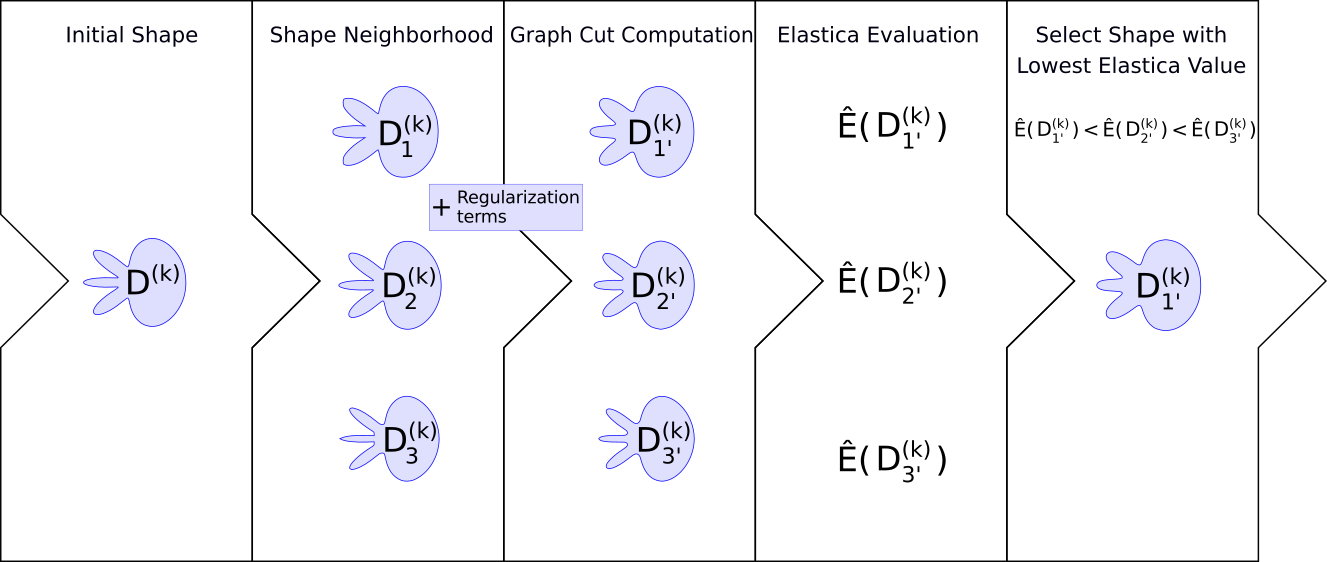
\includegraphics[scale=0.36]{figures/model-overview.png}
\caption{Proposed segmentation model. Our iterative segmentation model builds one graph for each member of a pre-defined
neighborhood of the current shape. A cost function is defined such that the minimum cut of the graphs reflect the
energy we aim to optimize with its desired regularization terms. In our experiments, we use regularization terms for 
data and curvature. Finally, we select the shape with minimum elastica value, estimated via a multigrid convergent 
estimator. The process is repeated for the selected shape and it stops after a fixed number of iterations.}
\label{fig:model-overview}
\end{figure}
%
%
%
%
%
\section{Estimation of geometric quantities on digital data}

Let $C:[0,t] \rightarrow \mathbb{R}^2$ a parameterized plane curve with continuous first and second derivatives. In this case, we can easily compute the curvature at some point $P(t) = \big( x(t),y(t) \big) \in C$ by using the formula

\begin{align*}
\kappa (t) &= \frac{y'(t)x''(t) -x'(t)y''(t)}{(x'(t)^2 + y'(t)^2)^{3/2}}.
\end{align*}

What about if we do not know the curve equation, but instead, we have a finite set of points that is an \emph{exact sampling} $C$ ? That is, a finite sequence $P$ is an {\em exact sampling} of $C$ whenever each element of $P$ is an element of $C$ and the order of the points in the sequence corresponds to the ordering of points $P$ when moving along $C$. In this case, we can approach the curve $C$ by a sequence of straight lines joining consecutive points of $P$ and estimate the curvature by computing the angle defect between consecutive lines. This estimation is convergent (in the epi-convergent sense) as long as the sampling points are sufficiently numerous~\cite{bruckstein01discrete,bruckstein01convergence}.

The result above is not valid for curves lying in digital domains like images. We do not have an exact sampling. Instead, curve samples are constrained to lie in the digital grid. That condition creates ambiguities, which are clearly illustrated in~\cref{fig:digitization-ambiguity} where the same digitization represents two quite distinct shapes. Of course, one may refine the grid to reach a precision close to an exact sampling, but this is highly undesirable due to memory and running time complexity, in particular for image processing tasks. Furthermore, the polygonal contour is still locally very jagged, with only 4 possible directions. The above mentionned curvature estimator would not be convergent whatever the refinement.

Consequently we need a criterion to evaluate the quality and speed
of convergence of geometric estimators according to the resolution of
the digital grid. This criterion is the \emph{multigrid convergence
property} (e.g., see \cite{klette2004digital}). Let $X$ be a Euclidean
shape and $\partial X$ its topological boundary. We further denote $D(X,h):=X \cap h\mathbb{Z}^2$ its Gauss digitization as a collection  of points, $Q(x,h)$ its pixel representation (a collection  of squares of side $h$), $\Delta_h X$ its interpixel contour as a collection  of axis aligned edge segments of length $h$, and finally $\partial_hX$ the digitized contour, which is the union of all edge segments of $\Delta_h X$. See \cref{fig-notations} for an illustration of notations.
%
%
\begin{figure}
\center
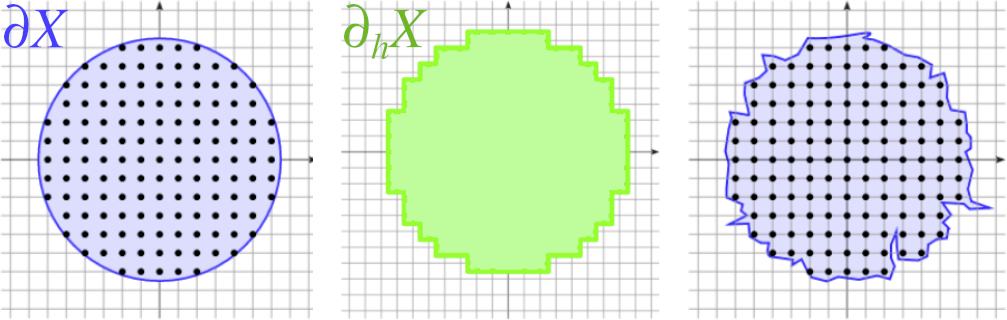
\includegraphics[scale=1]{figures/ambiguity-and-boundaries.png}
\caption{\textbf{Digitization ambiguity.} The middle image (in green) is a valid digitization for both the left and right continuous shapes (in blue).}
\label{fig:digitization-ambiguity}
\end{figure}
%
%
\begin{definition}[Multigrid convergence for local geometric quantites]
  A local discrete geometric estimator $\hat{z}$ of some geometric
  quantity $z$ is uniformly multigrid convergent for some family $\mathbb{X}$ of Euclidean shapes if
  and only if, for any $X \in \mathbb{X}$, there exists a grid step
  $h_X>0$ such that the estimate $\hat{z}(D(X,h), P,h)$ is
  defined for all $P \in \partial_hX$ with $ 0 < h < h_X$, and
  for any $Q \in \partial X$,
  \begin{equation*}
    \forall P \in  \partial_hX \text{ with } \norm{ P - Q }_{\infty} \leq h, \norm{ \hat{z}(D(X,h),P,h) - z(X,Q)} \leq \tau_{X}(h),			
  \end{equation*}
  where $\tau_{X}:\mathbb{R}^{+}\setminus\{0\} \rightarrow
  \mathbb{R}^{+}$ has null limit at $0$. This function defines the
  speed of convergence of $\hat{z}$ towards $z$ for $X$.
\end{definition}
	
For a global geometric quantity (e.g. perimeter, area, volume), the definition remains the same, except that the mapping
between $\partial X$ and $\partial_h X$ is no longer necessary.

\begin{figure}
  
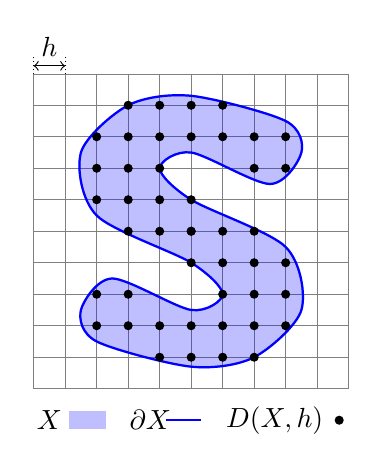
\begin{tikzpicture}[x=0.4cm,y=0.4cm]
  % grids
  \draw[help lines,step=0.4cm] (0,0) grid (10,10);
  % shape
  \draw[draw,thick,fill,color=blue,nearly transparent] plot[smooth cycle] 
            coordinates{(5,9.3) (8,8.5) (8.5,7.5) (7.5,6.5) (5,7.5) (4,7) (5,6) (8,4.5) (8.5,2.5) (7,1)
                        (5,0.7) (2,1.5) (1.5,2.5) (2.5,3.5) (5,2.5) (6,3) (5,4) (2,5.5) (1.5,7.5) (3,9)} -- cycle;
  % shape boundary          
  \draw[draw,thick,color=blue] plot[smooth cycle] 
            coordinates{(5,9.3) (8,8.5) (8.5,7.5) (7.5,6.5) (5,7.5) (4,7) (5,6) (8,4.5) (8.5,2.5) (7,1)
                        (5,0.7) (2,1.5) (1.5,2.5) (2.5,3.5) (5,2.5) (6,3) (5,4) (2,5.5) (1.5,7.5) (3,9)} -- cycle;
  % gauss digitization
  \foreach \x/\y in {3/9,4/9,5/9,6/9,2/8,3/8,4/8,5/8,6/8,7/8,8/8,2/7,3/7,4/7,7/7,8/7,2/6,3/6,4/6,5/6,3/5,4/5,5/5} {
    \draw[color=black,fill] (\x,\y) circle (0.5mm);
    \draw[color=black,fill] (10-\x,10-\y) circle (0.5mm);
  };
  % legend
  \node at(0.5,-1) {$X$};
  \node[rectangle,fill,color=blue,nearly transparent] at(1.7,-1) {\mbox{~~}};
  \node at(3.7,-1) {$\partial X$};
  \draw[draw,thick,color=blue] (4.2,-1) -- (5.3,-1);
  \node at(7.8,-1) {$D(X,h)$~~};
  \draw[color=black,fill] (9.7,-1) circle (0.5mm);
  \draw[densely dotted,black] (0,10) -- (0,10.6);
  \draw[densely dotted,black] (1,10) -- (1,10.6);
  \draw[<->,black] (0,10.25) -- (1,10.25) node[midway,above] {$h$};
\end{tikzpicture}
~
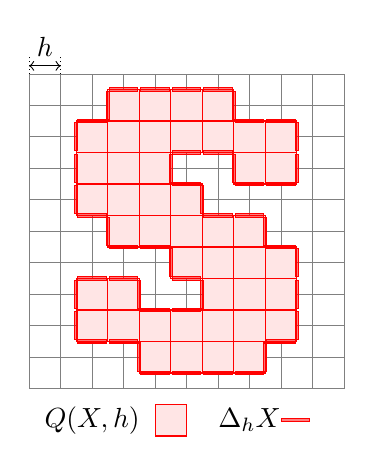
\begin{tikzpicture}[x=0.4cm,y=0.4cm]
  \draw[help lines,step=0.4cm] (0,0) grid (10,10);
  % QhZ
  \foreach \x/\y in {3/9,4/9,5/9,6/9,2/8,3/8,4/8,5/8,6/8,7/8,8/8,2/7,3/7,4/7,7/7,8/7,2/6,3/6,4/6,5/6,3/5,4/5,5/5} {
    \draw[color=red!10!white,fill] (\x-0.5,\y-0.5) rectangle (\x+0.5,\y+0.5);
    \draw[draw,thin,color=red] (\x-0.5,\y-0.5) rectangle (\x+0.5,\y+0.5);
    \draw[color=red!10!white,fill] (10-\x-0.5,10-\y-0.5) rectangle (10-\x+0.5,10-\y+0.5);
    \draw[draw,thin,color=red] (10-\x-0.5,10-\y-0.5) rectangle (10-\x+0.5,10-\y+0.5);
  };
  % horizontal boundary edges
  \foreach \x/\y in {3/9,4/9,5/9,6/9,7/8,8/8,8/6,7/6,6/7,5/7,5/6,6/5,7/5,8/4,8/1} {
    \draw[color=red,fill,opacity=0.5] (\x-0.45,\y+0.45) rectangle (\x+0.45,\y+0.55);
    \draw[draw,color=red] (\x-0.45,\y+0.45) rectangle (\x+0.45,\y+0.55);
    \draw[color=red,fill,opacity=0.5] (10-\x-0.45,9-\y+0.45) rectangle (10-\x+0.45,9-\y+0.55);
    \draw[draw,color=red] (10-\x-0.45,9-\y+0.45) rectangle (10-\x+0.45,9-\y+0.55);
  }
  % vertical boundary edges
  \foreach \x/\y in {6/9,8/8,8/7,6/7,4/7,5/6,7/5,8/4,8/3,8/2,7/1} {
    \draw[color=red,fill,opacity=0.5] (\x+0.45,\y-0.45) rectangle (\x+0.55,\y+0.45);
    \draw[draw,color=red] (\x+0.45,\y-0.45) rectangle (\x+0.55,\y+0.45);
);
    \draw[color=red,fill,opacity=0.5] (9-\x+0.45,10-\y-0.45) rectangle (9-\x+0.55,10-\y+0.45);
    \draw[draw,color=red] (9-\x+0.45,10-\y-0.45) rectangle (9-\x+0.55,10-\y+0.45);
);
  }
  %% \node at(0.5,-1) {$X$};
  %% \node[rectangle,fill,color=blue,nearly transparent] at(1.7,-1) {\mbox{~~}};
  \node at(2,-1) {$Q(X,h)$};
  \draw[color=red!10!white,fill] (4,-1.5) rectangle (5,-0.5);
  \draw[thin,draw,color=red] (4,-1.5) rectangle (5,-0.5);
  \node at(7,-1) {$\Delta_h X$};
  \draw[color=red,fill,opacity=0.5] (8,-0.95) rectangle (8.9,-1.05);
  \draw[draw,color=red] (8,-0.95) rectangle (8.9,-1.05);
  \draw[densely dotted,black] (0,10) -- (0,10.6);
  \draw[densely dotted,black] (1,10) -- (1,10.6);
  \draw[<->,black] (0,10.25) -- (1,10.25) node[midway,above] {$h$};
\end{tikzpicture}
~
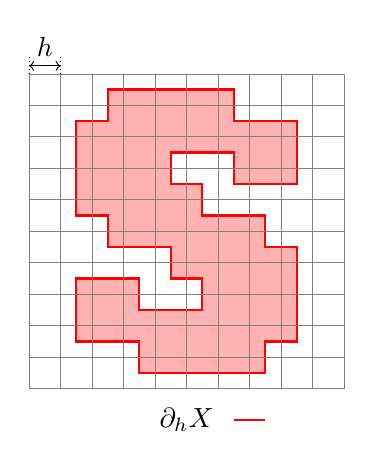
\begin{tikzpicture}[x=0.4cm,y=0.4cm]
  % QhZ
  \foreach \x/\y in {3/9,4/9,5/9,6/9,2/8,3/8,4/8,5/8,6/8,7/8,8/8,2/7,3/7,4/7,7/7,8/7,2/6,3/6,4/6,5/6,3/5,4/5,5/5} {
    \draw[color=red!30!white,fill] (\x-0.5,\y-0.5) rectangle (\x+0.5,\y+0.5);
    \draw[color=red!30!white,fill] (10-\x-0.5,10-\y-0.5) rectangle (10-\x+0.5,10-\y+0.5);
  };
  % \partial_h X
  \draw[color=red,thick] (2.5,9.5) -- (6.5,9.5) -- (6.5,8.5) -- (8.5,8.5) -- (8.5,6.5) -- (6.5,6.5)
                             -- (6.5,7.5) -- (4.5,7.5) -- (4.5,6.5) -- (5.5,6.5) -- (5.5,5.5) -- (7.5,5.5) 
                             -- (7.5,4.5) -- (8.5,4.5) -- (8.5,1.5) -- (7.5,1.5) -- (7.5,0.5) -- (3.5,0.5)
                             -- (3.5,1.5) -- (1.5,1.5) -- (1.5,3.5) -- (3.5,3.5) -- (3.5,2.5) -- (5.5,2.5)
                             -- (5.5,3.5) -- (4.5,3.5) -- (4.5,4.5) -- (2.5,4.5) -- (2.5,5.5) -- (1.5,5.5)
                             -- (1.5,8.5) -- (2.5,8.5) -- cycle;
  % grids
  \draw[help lines,step=0.4cm] (0,0) grid (10,10);
  %  \node at(2.5,-1) {$\Body{DSh}{h}$~~};
  %\node[color=red!30!white,fill] at(4.5,-1) {\mbox{~~}};
  \node at(5,-1) {$\partial_h X$};
  \draw[color=red,thick] (6.5,-1) -- (7.5,-1);
  \draw[densely dotted,black] (0,10) -- (0,10.6);
  \draw[densely dotted,black] (1,10) -- (1,10.6);
  \draw[<->,black] (0,10.25) -- (1,10.25) node[midway,above] {$h$};
\end{tikzpicture}

  \caption{Illustration of notations: the shape $X$, its topological boundary $\partial X$, its (Gauss) digitization $D(X,h)=X \cap h \Z^2$ seen as a collection of points, its pixel representation $Q(X,h)$ which is a set of squares of side $h$, the interpixel contour $\Delta_h X$ as a set of axis-aligned edge segments, and the digitized boundary $\partial_h X$, a subset of $\R^2$ that is the union of all edges of the interpixel contour, or equivalently the topological boundary of the union of all the squares of $Q(X,h)$.\label{fig-notations}}
\end{figure}

Recently, estimator for curvature and perimeter estimators have been proved multigrid convergent. We propose to use such estimators to estimate the elastica energy of digital shapes. Let us define a digital analogue to the Elastica energy, which uses two such estimators:
%
%
\begin{align}
	\hat{E}_r\big( D(X,h),h,\alpha,\beta) \big) = \sum_{e \in \Delta_h X}{ \hat{s}(e)\left(\; \alpha + \beta \hat{\kappa}_{r}^2(D(X,h),\dot{e},h) \; \right)}.
	\label{eq:digital-energy}
\end{align}
%
%
The symbol $\dot{e}$ denotes the center of the edge $e$.  The
function $\hat{s}$ denotes the elementary length estimator, i.e., a
measure of length is assigned to each edge $e$ of the digital curve
$\Delta_h X$. The elementary length is computed using the
\emph{$\lambda$-MST} estimator of
tangent~\cite{lachaud07tangent,lachaud06hdr}, proven multigrid
convergent for the family of convex shapes that are twice
differentiable and have continuous curvature. The speed of convergence
is $O(h^{1/3})$. It simply defines the elementary
  length of an edge as the scalar product between the edge vector and
  the convergent tangent vector estimate.

The function $\hat{\kappa} _r$ denotes an estimator of curvature. We use the integral \emph{invariant estimator}~\cite{coeurjolly13integral}, proven multigrid convergent for the family of compact shapes in the plane with $3$-times differentiable contour. The radius of the integration ball is a parameter of this curvature estimator and its convergence speed is of the order of $O(h^{\frac{1}{3}})$ for radii chosen as $r=\Theta (h^{\frac{1}{3}})$~\cite{lachaud2017robust}. We present its definition since it is at the core of the model proposed in this paper.
%
%
\begin{align}
  \tilde{\kappa}_r(D(X,h),P,h) \coloneqq \frac{3}{r^3}\left( \frac{\pi r^2}{2} - \widehat{\text{Area}}\big( D(B_r(P),h) \cap D(X,h),h\big) \right),
  \label{eq:curvature_approximation}
\end{align}
%
%
where the estimation of area for some digital set $S$ is defined as $\widehat{\text{Area}}(S,h) \coloneqq h^2\text{Card}\left( S \right).$ 

\Cref{eq:curvature_approximation} estimates the curvature as a scaling factor of the difference between the intersection area of the digitized shape with a disk of radius $r$ centered at point $P$ of the contour and half the disk area. Therefore, we can say that the curvature is lower at points in which the balance between intersected and non intersected points is closer to zero.

In the following, we simply write $S$ to specify a digital shape and we omit the grid step $h$ to simplify expressions (or, putting it differently, we assume that the shape of interest is rescaled by $1/h$ and we set $h = 1$).
%
%
%
%
%
\section{Balance coefficient and curve-shortening flow}
%
%
\begin{figure}
 \center
 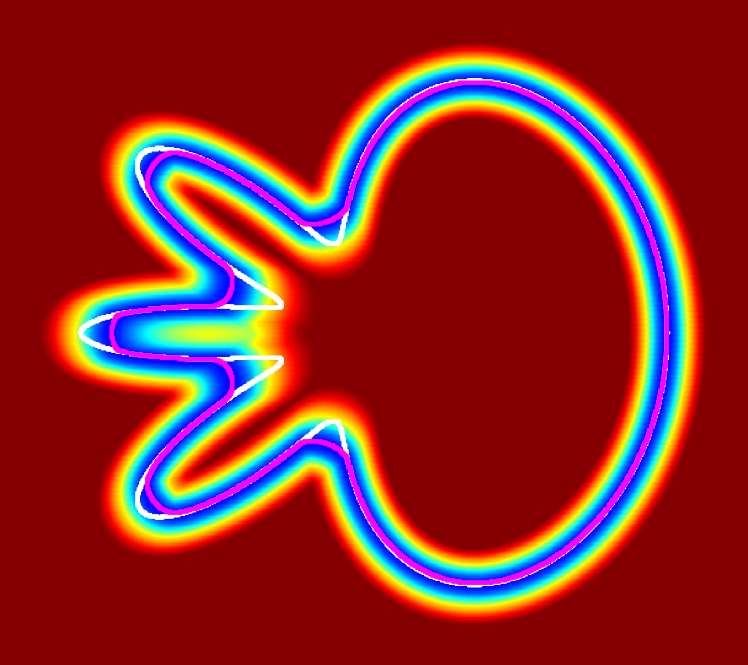
\includegraphics[scale=0.32]{figures/zero-level-set/balance-coefficient-zero-level-set.png}
 \caption{\textbf{Balance coefficient zero-level set}. Evolving the initial contour (colored in white) to the zero-level set of the balance coefficient (colored in black) is closeley related with the curve-shortening flow.}
 \label{fig:balance-coefficient-zero-level-set}
 \end{figure}
%
%
Let $X \subset \R^2$ be a Euclidean shape, $r$ a positive real number and $P$ an arbitrary point of $\R^2$. We define the \emph{balance coefficient $u_r$} of $X$ at $P$ as
%
%
\begin{align*}
  u_r(X,P) &= \left( \frac{\pi r^2}{2} - \text{Area}(B_r(P) \cap X) \right).
\end{align*}
%
%
We observe that the balance coefficient definition is similar to the
integral invariant estimator of curvature in
equation~\eqref{eq:curvature_approximation} (we can model the
continuous domain as a digital domain with an infinitely small grid
step). However, we do not use it to estimate the curvature, but rather
as an indicator of the local degree of convexity of the shape, even for points distant to the shape boundary.

In the following, we use the balance coefficient to define the balance
coefficient flow and we show how it relates with the curve-shortening
flow (CSF), the one-dimensional version of the mean curvature flow.

\begin{definition}[Balance coefficient flow]
  Let $X \subset \Omega$ be a Euclidean shape and $r>0$ the radius of the disk used to compute the balance coefficient. We define the \emph{balance coefficient flow} for discrete time steps as the sequence of Euclidean shapes
%
%
\begin{align}
  X^{(0)} & := X, \nonumber \\
  \forall k \in \Z, k > 0, \quad X^{(k+1)} & := \left\{ x \in \Omega \: | \: u_r(X^{(k)}, x) \leq 0 \right\}. \label{eq-balance-coefficient-flow}
\end{align}
%
%
\end{definition}
%
%
 One iteration of the balance coefficient flow applied on shape $X$ is equivalent to find the shape $X'$ such that for any disk of radius $r$ centered at any point of the contour of $X'$, the intersection of the disk with the shape $X$ equals $\pi r^2/2$. This interpretation is illustrated in~\cref{fig:geometric-interpretation}.
%
% 
\begin{figure}
\center
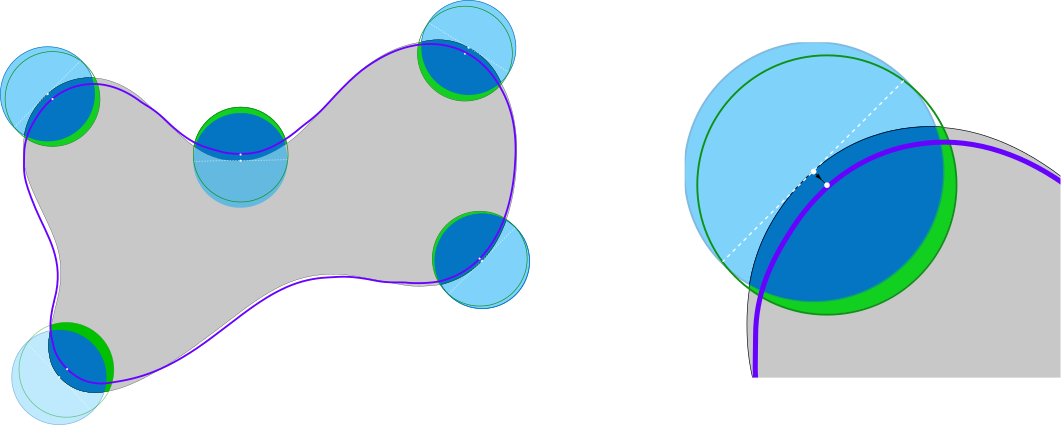
\includegraphics[scale=0.25]{figures/zero-level-set/geometric-interpretation.png}
\caption{\textbf{Geometric interpretation of the balance coefficient flow.} A single iteration of the balance coefficient flow evolves the shape $X$ to the shape $X'$ such that any disk of radius $r$ centered at any point of the contour of $X'$ intersects  an area of $\pi r^2/2$ of the initial shape $X$.}
\label{fig:geometric-interpretation}
\end{figure}
% 
%

Let us show the link between the balance coefficient flow and the
curve-shortening flow. First we rewrite the balance coefficient flow
as a contour evolution. Let us denote $C^{(0)} := \partial
X^{(0)}$ the boundary of $X^{(0)}$. Then, for $x \in C^{(0)}$,
let $\epsilon^{(0)}(x)$ be a solution to the equation
\begin{align} \label{eq-null-balance-coefficient}
  u_r(X^{(0)}, x +\epsilon^{(0)}(x)
  \mathbf{n}^{(0)}(x)) & = 0, \\
  |\epsilon^{(0)}(x)| & < r, \nonumber
\end{align}
with $\mathbf{n}^{(0)}(x)$ the outward normal vector at $x$ to
the boundary of the shape $X^{(0)}$. Specifying
$|\epsilon^{(0)}(x)| < r$ clearly imposes a unique solution to
~\cref{eq-null-balance-coefficient}, provided $r < 1/\kappa$. Then the
contour evolution of $C^{(0)}$ is defined as:
\begin{align} \label{eq-balance-coefficient-contour-flow}
  C^{(1)} := \left\{ \sigma^{(0)}(x), x \in C^{(0)} \right\},
\end{align}
where $\sigma^{(0)}$ is the mapping from $C^{(0)}$ to $C^{(1)}$, such that $x$ maps to $x+\epsilon^{(0)}(x) \mathbf{n}^{(0)}(x)$.

The following proposition indicates that $C^{(1)}$ coincides with
the boundary of $X^{(1)}$ under some hypotheses.

\begin{proposition} \label{prop-C-equ-X}
  If $r$ is small enough, the boundaries of shapes $X^{(0)}$ and
  $X^{(1)}$ are Jordan curves, and the boundary of shape $X^{(0)}$ is
  twice differentiable, then $C^{(1)}$ is the boundary of $X^{(1)}$,
  and the mapping $\sigma^{(0)}$ between $C^{(0)}$ and $C^{(1)}$ is
  bijective.
\end{proposition}
\begin{proof}
  By definition, the curve $C^{(0)}$ is the boundary of shape
  $X^{(0)}$.  Being twice differentiable the curve $C^{(0)}$ has a
  reach that is greater than some $\rho > 0$.\footnote{Let us recall
  recall that the {\em reach} is the infimum distance between a shape
  and its medial axis. Any point within the reach has a unique closest
  point to the shape by definition.} Hence, any point at distance lower than $\rho$
  from $C^{(0)}$ has a unique closest point on this curve, in the
  direction normal to the curve.

  Let $x$ be a point on $C^{(1)}$ and let
  $y=\sigma^{(0)}(x)=x+\epsilon^{(0)}(x) \mathbf{n}^{(0)}(x)$.
  Obviously, the smaller is $r$, the closer is $C^{(1)}$ from
  $C^{(0)}$.  From the definition of balance coefficient, one can see
  that the displacement that is solution to~\cref{eq-null-balance-coefficient} cannot exceed $\frac{1}{2}\kappa
  r^2$. So if $r < \sqrt{2\rho / \kappa_{\max}}$, where
  $\kappa_{\max}$ is the maximum absolute curvature of the curve, then
  the point $y$ is within the reach of the curve $C^{(0)}$. It follows
  that the mapping $\sigma^{(0)}$ is bijective. It is also continuous
  since all functions are continuous (the area of the shape
  intersected by a ball is continuous with respect to a displacement
  of the ball center).  Hence $C^{(1)}$ is a Jordan curve within the
  reach of $C^{(0)}$. It has therefore an interior component $I$.

  It is clear also that $y \in X^{(1)}$ since $u_r(X^{(0)},y)=0$.
  Let us denote $z(\lambda)=(1-\lambda)x+\lambda y$.

  If $u_r(X^{(0)},x)<0$ then $u_r(X^{(0)},z(\lambda))$ is by
  construction strictly increasing for increasing values of $0 \le
  \lambda \le 1+\nu$, $\nu \ll 1$, and so becomes positive for
  $1<\lambda < 1 + \nu$. In this case $C^{(0)}$ was concave at $x$,
  so the straight segment $\lbrack x,y \rbrack$ is included in
  $X^{(1)}$ and $y$ lies on its boundary. We have also $X^{(1)}
  \cap \lbrack x,y \rbrack \subset I$, and $x$ lies in the interior of
  $X^{(1)}$.
  
  If $u_r(X^{(0)},x)>0$ then $u_r(X^{(0)},z(\lambda))$ is by
  construction strictly decreasing for increasing values of $0 \le
  \lambda \le 1+\nu$, $\nu \ll 1$, and so becomes negative for
  $1<\lambda < 1 + \nu$.  In this case $C^{(0)}$ was convex at $x$,
  so the straight segment $\lbrack x,y \lbrack$ is excluded from
  $X^{(1)}$ and $y$ lies on its boundary. We have also $X^{(1)}
  \cap \lbrack x(1),x(1+\nu) \rbrack \subset I$ and $x(1+\nu)$ lies in
  the interior of $X^{(1)}$.

  In both case we can see that $y$ lies on the boundary of
  $X^{(1)}$. So $C^{(1)} \subset \partial X^{(1)}$. Since both
  are Jordan curves they must coincide and $C^{(1)} = \partial
  X^{(1)}$.  Finally, the interior of $X^{(1)}$ must coincide with
  $I$ since both are finite, they share the same boundary, and they
  share points (whether the boundary is convexe or concave).
  %% \qed %% does not work
  %% \hfill $\square$
\end{proof}

The proof tells us that the radius $r$ must be smaller that
$\min(\sqrt{2\rho / \kappa_{\max}},2 / \kappa_{\max})$, for $\rho>0$
smaller than the reach of the shape and $\kappa_{\max}$ the maximal
absolute curvature of the shape.

Let us recall that the curve-shortening flow for a small time step
$t>0$, may be defined as:
\begin{align}
  \Gamma^{(0)} & := \partial X \nonumber \\
  \Gamma^{(t)} & := \left\{ x + t\kappa(x)\mathbf{n}(x), x \in \Gamma^{(0)} \right\}, \label{eq-csf}
\end{align}
denoting by $\kappa(x)$ the curvature of the curve at point $x$
and by $\mathbf{n}(x)$ the outward normal vector at $x$.

Of course, there are implicitly defined variants of this formulation
that allows topology changes, but we will restrict ourselves here to
proving the similarity between the balance coefficient flow and the
curve-shortening flow when there is no topology change.


%
\begin{figure}
\center
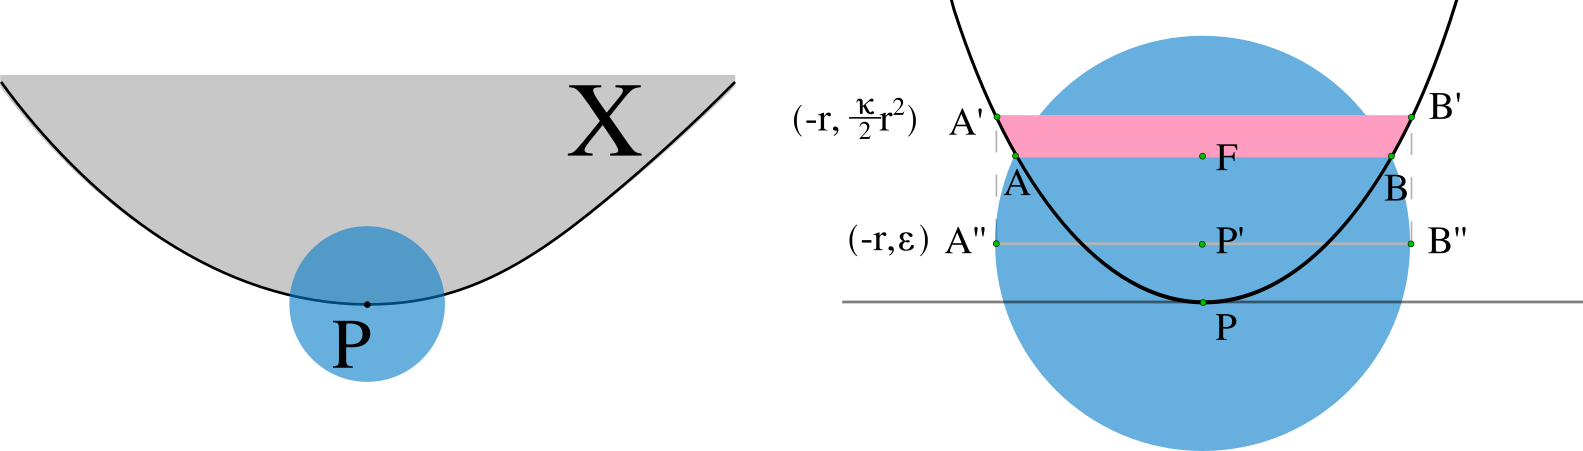
\includegraphics[scale=0.75]{figures/analysis-error/geometry-argument.png}
\caption{\textbf{Balance coefficient and curve-shortening flow (CSF).} We approximate the contour $\partial X$ at $P$ by a parabola. Next, we compute the point $P'$ such that the balance coefficient equals to zero. Our approximation produces an error $\Delta$, highlighted in magenta, that is of order $O(r^4)$. \label{fig:geometric-argument}}
\end{figure}
%

\begin{proposition}\label{prop:bcf-close-to-csf}
  For small enough $r$, setting $t = \frac{1}{6}r^2$, assuming $C^{(0)}=\Gamma^{(0)}$ is a twice differentiable Jordan curve, then the Hausdorff distance between
  $C^{(1)}$ and $\Gamma^{(t)}$ is some $O(t^2)$, more precisely we get:
  \begin{align*}
    d_H( C^{(1)}, \Gamma^{(t)} ) \le \frac{3}{4} \kappa_{\max}^3 t^2.
  \end{align*}
\end{proposition}
\begin{proof}
  Let $y \in C^{(1)}$. According to~\cref{prop-C-equ-X},
  there is a point $P \in C^{(0)}$ such that
  $y=\sigma^{(0)}(P)$. Let $y'=P+t\kappa(P)\mathbf{n}(P)$. We
  show that $\| y-y' \| \le \frac{3}{4} \kappa_{\max}^3 t^2$,
  which induces the result (we could have chosen $y'$ first, and
  obtain the same $y$).

  We center the reference frame on $P$ with $y$-axis aligned with the
  normal vector $\mathbf{n}(P)$.  Since $r$ is small enough, the
  contour is well approximated by the parabola $f(x) :=
  \frac{\kappa(P)}{2}x^2$ in this frame.

  We know that $y = P + \epsilon^{(0)}(P)\mathbf{n}(P)$ according
  to~\cref{eq-null-balance-coefficient}, where $\epsilon^{(0)}(P)$ is
  the local displacement of $P$ which gives a zero balance
  coefficient. Let us determine this displacement $\varepsilon :=
  \epsilon^{(0)}(P)$ in the normal direction, such that the
  intersection of the disk with $X$ equals half of the disk area. Let
  us say that the point of zero balance coefficient is $P'$ and that
  $A_{\varepsilon}$ is the intersection area of the displaced disk
  (see~\cref{fig:geometric-argument}, right, for
  notations). Then,
%
%
\begin{align*}
	 & A_{\varepsilon} = \frac{\pi r ^2}{2} 
	 && \Rightarrow & 2r\varepsilon = \int_{-r}^{r}{\frac{1}{2}\kappa x^2dx} \pm \Delta 
	&& \Leftrightarrow & & \varepsilon = \frac{1}{6}\kappa r^2 \pm \frac{\Delta}{2r}.
\end{align*}
%
%
It remains to compute an upper bound for the error $\Delta$. Let $A^3$ be the leftmost intersection point between the line $A'B'$ and the estimation disk. It is clear that $\Delta/2$ is smaller than the region between $A''A'A^3$ and the arc going from $A^3$ to $A''$. Let $d$ be the length of the segment $A'A''$. 
%
%
\begin{align*}
	Area(A''A'A^3) &= \int_0^d{r - \sqrt{r^2 - x^2} dx} \\
				   &= -\frac{r^2}{2}sin^{-1}\left(\frac{d}{r}\right) + dr - \frac{d}{2}\sqrt{r^2-d^2} \\
				   &\approx \frac{d^3}{6r}.
\end{align*}
%
%
In general, $d$ is bounded by $\frac{1}{2}\kappa r^2$, hence it follows:
%
%
\begin{align*}
	\frac{\Delta}{2} \leq \frac{d^3}{6r} \leq \frac{1}{48}\kappa^3r^5.
\end{align*}
%
%
Therefore,
%
%
\begin{align*}
	\varepsilon &= \frac{1}{6}\kappa r^2 \pm \frac{1}{48}\kappa^3r^4.
\end{align*}
%
%
To conclude the argument, we have:
\begin{align*}
  \| y - y' \| & = \| P + \epsilon^{(0)}(P)\mathbf{n}(P) - (P+t\kappa(P)\mathbf{n}(P)) \| \\
  & = | \varepsilon - t \kappa(P) | \\
  & \le \left| \frac{1}{6}\kappa(P) r^2 - t\kappa(P) \right| + \frac{1}{48}|\kappa(P)|^3r^4\\
  & \le \frac{1}{48}|\kappa(P)|^3r^4 && \text{(since $t=\frac{1}{6}r^2$)} \\
  & \le \frac{3}{4}\kappa_{\max}^3 t^2 && \text{(since $|\kappa(P)| \le \kappa_{\max}$)}
\end{align*}
which shows that the two contours are close in the Hausdorff sense.
\end{proof}

Applying~\cref{prop-C-equ-X} at each time step $k$ (writing
$(k)$ instead of $(0)$ and $(k+1)$ instead of $(1)$) allows us to
redefine the balance coefficient flow as the sequence $C^{(k)}$,
provided that the boundaries of $X^{(k)}$ are twice differentiable
Jordan curves. But~\cref{prop:bcf-close-to-csf} applied on
these consecutive curves tells us that the curves $C^{(k)}=\partial
X^{(k)}$ are very close to the curve shortening flow, which induces
twice differentiable curves except at critical points. Proving that
the flow $X^{(k)}$ also mimicks the curve-shortening flow across
critical points would require much more mathematical work and is
outside the scope of this paper.

The CSF has many interesting properties~\cite{huisken84flow,gage86heat,ecker2008heat}. Among those, the CSF is the continuous deformation that decreases the perimeter of a single closed curve at the fastest speed; and it also preserves convexity. In particular, the CSF eventually collapses the initial curve to a single point.

There are interesting links between the CSF and a variant of the heat equation defined for the indicatrix function of a set~\cite{merriman1992diffusion}. In this same work, the authors informally give a geometric interpretation for the CSF that is equivalent to our zero-level set of the balance coefficient. A technique that emerged from the interpretation of CSF as a heat equation is the so called threshold dynamics~\cite{esedoglu2005threshold,esedoglu2008threshold}. However, the use of threshold dynamics for image processing tasks is not immediate due to the difficulty to inject a data fidelity term. That is not the case in our approach.

We are going to apply the balance coefficient flow in a discrete setting. In theory, that means that we have some limitations regarding the choice of the estimation radius $r$, the grid resolution $h$ and the real curvature value at the estimation point. In general, we need to respect
%
%
\begin{align*}
	h \ll r \ll \frac{1}{\kappa}.
\end{align*}
%
%
In practice, we are going to show that we can achieve good results without being too strict regarding the restriction above.
%
%
%
%
\section{Elastica minimization of digital shapes via graph cuts}
We recall our estimator for the elastica energy 
%
\begin{align}
	\hat{E}_{\Theta}\big( S \big) = \sum_{\vec{e} \in \partial S}{ \hat{s}(\vec{e})\left(\; \alpha + \beta \hat{\kappa}_{r}^2(S,\dot{\vec{e}}) \; \right)}.
	\label{eq:elastica-estimator-2}
\end{align}
%
%
Notice that we group all parameters in vector $\vec{\Theta}=(h,r,\alpha,\beta)$. We remark that, since it is composed of multigrid convergent estimators, the elastica estimator is also multigrid convergent~\cite{lachaud06hdr}.

In this section we describe a graph cut model for the optimization of digital shapes with respect to the elastica energy. The model can be divided in three
parts. In the first part, we define a neighborhood of shapes with respect with the given digitized object. Next, for each shape in the neighborhood 
we create a candidate graph. A graph-cut optimization is done in each candidate graph and the result of each optimization gives us a candidate shape. Finally, we compute the elastica on the candidate shapes and select the one with lowest elastica value.
%
%
\subsection{Neighborhood of shapes}
%
%
We start by defining a very simple neighborhood of shapes. Of course, richer neighborhoods could be used, but we
stick here to this elementary one, which will prove to be sufficient in our experiments.
%
%
\begin{definition}[Neighborhood of shapes]
	Let $S \subset \mathbb{Z}^2$ a digital shape. We define its {\em neighborhood}  $\mathcal{N}(S)$ as the set
	\begin{align*}
		\mathcal{N}(S) &= \Big\{S, S^{+1},S^{-1} \big\},
	\end{align*}
	where $S^{+1}$ ($S^{-1}$) denotes a morphologic dilation (erosion) by a square of side $1$.
\end{definition}
%
%
\subsection{Computation of candidates}\label{sec:graph-cut-model}

We are going to define a directed weighted graph and set its edge weights
such that we can evolve the shape towards the zero-level set of
its balance coefficient. Since the balance
coefficient is a local quantity, it is sufficient to define the graph
in a band around the initial contour. This somewhat
  complex approach to computing a zero-level set of a function has the
  great advantage of allowing the integration of other terms in its
  formulation, like fitting to data. Experiments will show that it has
  a tremendous effect on the quality of image segmentation results.

Let $d_{S}:\Omega \rightarrow \mathbb{R}$ be the signed Euclidean distance transformation with respect to shape $S$. The value $d_{S}(P)$ gives the Euclidean distance between $P \notin S$ and the closest point in $S$. For points $P \in S$, $d_{S}(P)$ gives the negative of the distance between $P$ and the closest point not in $S$. Let $n$ be a positive integer number.

\begin{definition}[Optimization band]
Let $S \subset \Omega \subset \mathbb{Z}^2$ be a digital set
. The optimization band
$O_n(S)$ is defined as
%
%
\begin{align*}
	O_n(S) &:=\left\{ P \in \Omega \; | \; -n \leq d_{S}(P) \leq n \right\}.
\end{align*}
\end{definition}
%
%
\begin{definition}[Candidate graph]
Let $S \subset \Omega \subset \mathbb{Z}^2$ a digital set. The {\em candidate graph} $\mathcal{G}(n,S,\mathcal{V},\mathcal{E})$ of $S$ with optimization band $n$ is defined such that:
%
%
\begin{align*}
\mathcal{V} &= \big\{\; v_P \; | \; P \in O_n(S) \;\} \cup \{s,t \big\}, \\
\mathcal{E} &= \mathcal{E}_u \cup \mathcal{E}_{st}, \\
\mathcal{E}_u &= \big\{ \; \{v_P,v_Q\} \; | \; P \in O_n(S) \text{ and } Q \in \mathcal{N}_4(P) \; \big\}, \\
\mathcal{E}_{st} &= \big\{\; \{s,v_P\} \; | \; d_S(P)=-n \; \big\} \cup \big\{\; \{v_P,t\} \; | \; d_S(P)=n \; \big\}.
\end{align*}
%
%
\end{definition}

The vertices $s,t$ are virtual vertices representing the source and target vertices as it is common in a minimum cut framework. We denote $\mathcal{N}_4(P)$ the set of $4$-adjacent neighbors of $P$. The innermost (outermost) pixels of the optimization band are connected to the source (target), and we identify such vertices as
%
%
\begin{align*}
	\mathcal{V}_s &:=\left\{ v_P \in \Omega \; | \; d_{S}(P) = -n \right\}, \\
	\mathcal{V}_t &:=\left\{ v_P \in \Omega \; | \; d_{S}(P) = n \right\}.
\end{align*}
%
%
The set $\mathcal{E}_{st}$ comprises all the edges having the source as their starting point or the target as their endpoint. In~\cref{tab:edge-capacity} we describe the edge capacity function.
%
%
\begin{table}
\footnotesize
	\caption{\textbf{Edge capacity function.} $M$ is defined as $\max_{e \in \mathcal{E} }{ c(e) }$.}\label{tab:edge-capacity}
\begin{center}
\begin{tabular}{|c|c|c|}
\hline
\textbf{edge} $e$ & $\mathbf{c(e)}$ & \textbf{for}\\
\hline
$\{v_P, v_Q\}$ & $ \frac{1}{2}\left( u_r(S,P) + u_r(S,Q) \right) $ & $\{v_P,v_Q\} \in \mathcal{E}_{u}$\\
\hline
$\{v_P, s\}$ & $M$ & $v_P \in \mathcal{V}_{s}$ \\
\hline
$\{v_P, t\}$ & $M$ & $v_P \in \mathcal{V}_{t}$ \\
\hline
\end{tabular}
\end{center}
%% ,where $M$ is defined such that
%% %\begin{align*}
%% %	M &= 1+\max_{p \in O_n(S)} 2*u(S,h,r,p).
%% %\end{align*}
%% \begin{align*}
%% 	M &= \max_{e \in \mathcal{E} }{ c(e) }.
%% \end{align*}
\end{table}
%
%

A cut in a graph separates the vertices in source and target components. Our model is defined such that the source component of the minimum cut gives the next shape in balance-coefficient flow. 
%In other words, let $mincut(\mathcal{G})$ denote the source component of the minimum cut of capacitated graph $\mathcal{G}$.

%Then, we define
%
%
%\begin{align}
%	\forall t \geq0, \quad S^{(t+1)} = mincut\left( \mathcal{G}(S^{(t)}) \right), 
%	\label{eq:no-neighborhood-process}
%\end{align}
%
%
%where $S^{(0)}$ is the initial shape.\comment[id=jaco]{May be misleading for the whole process since there are several candidate graphs at each step.} Here and in the following, we omit some parameters of the candidate graph to simplify notation. They are going to be explicitly defined if necessary.

\subsection{Candidate Selection}
%
%
The graph-cut optimization applied to each candidate graph results in a candidate shape. At this step, we simply compute the elastica energy on each 
candidate shape using~\cref{eq:elastica-estimator-2} and then we select the candidate with lowest elastica value.


In~\cref{fig:no-neighborhood-shapes-evolution}, we show some examples of this process. As expected, the flow is very similar to the CSF. 
% Next, we describe how to optimize the shape with respect to the elastica energy by using a neighborhood of shapes.
%% \added[id=jaco]{More precisely, the graph cut is performed on several candidate graphs, one for each shape in a neighborhood of shapes, and the best one according to the elastica energy is selected.}
%
%
%
\begin{figure}
	\center
	\subfloat[]{%
	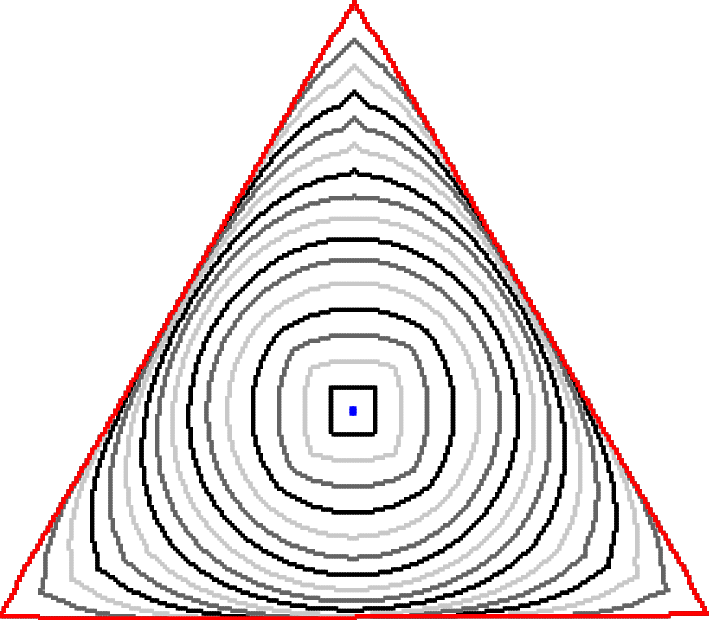
\includegraphics[scale=0.12]{figures/no-neighborhood-flow/triangle.png}}\hspace{2em}%
	\subfloat[]{%
	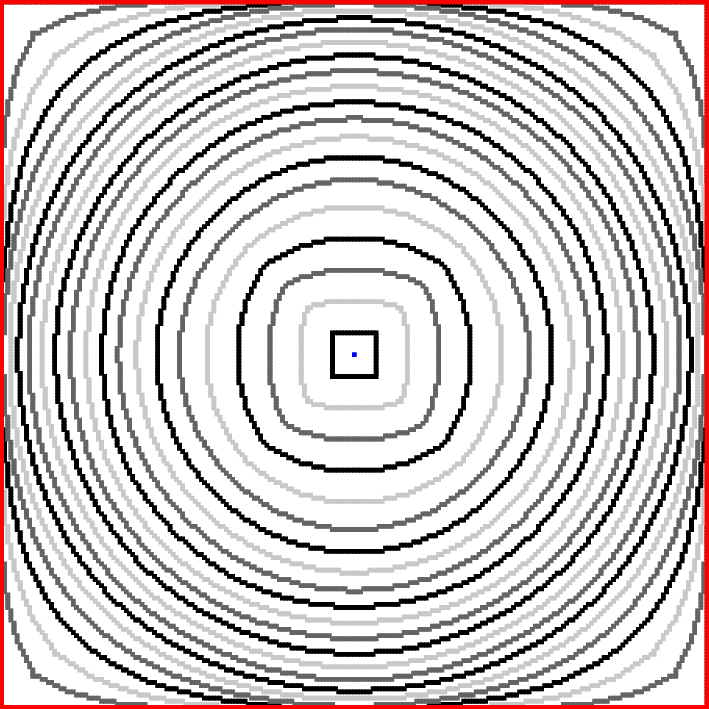
\includegraphics[scale=0.11]{figures/no-neighborhood-flow/square.png}}\hspace{2em}%	
	\subfloat[]{%
	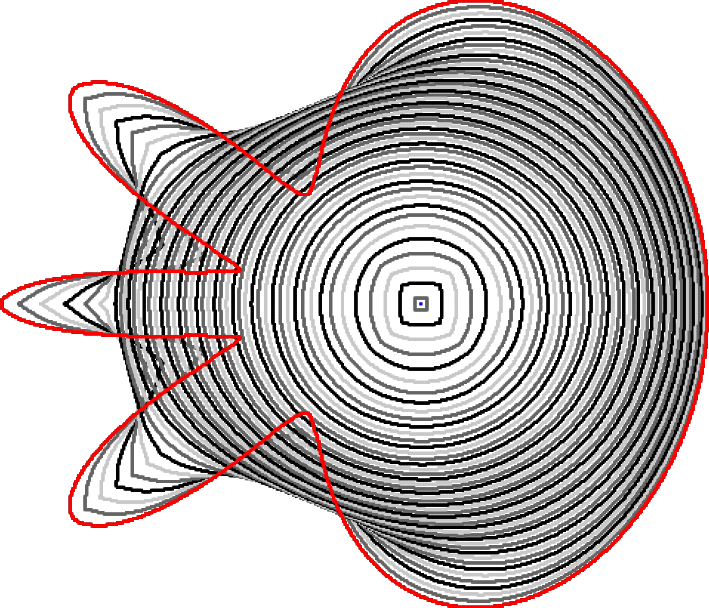
\includegraphics[scale=0.14]{figures/no-neighborhood-flow/flower.png}}	
	\caption{\textbf{No neighborhood of shapes}. Evolution with no neighborhood of shapes defined $(h=1/8,r=2)$. The evolution mimicks the curve-shortening flow. Initial contour is colored in red and each other contour is ploted every 10 iterations.}
	\label{fig:no-neighborhood-shapes-evolution}
\end{figure}
%
%
%
%
%
%
The {\em Graph Flow Algorithm} (GFA), Algorithm~\ref{alg:graphflow-algorithm}, summarizes the process. Some experiments are shown on \cref{fig:graph-flow-experiments} and \cref{fig:graph-flow-expand}.
%
%
\begin{algorithm}
 \caption{Graph Flow Algorithm (GFA).}
 \label{alg:graphflow-algorithm}  
\begin{algorithmic} 
 \STATE{\textbf{Input}: A digital set $S$; the optimization band $n$; parameter vector $\vec{\theta}=(h,r,\alpha,\beta)$; the maximum number of iterations $maxIt$;} 
 
 \STATE{$S^{(0)} \longleftarrow S$}
 \STATE{$t \longleftarrow 0$}
 \WHILE{ $t$ $<$ $maxIt$  } 	
	\STATE{$\mathcal{C}^{(t)} \longleftarrow \bigcup_{S' \in \mathcal{N}(S^{(t)})} \Big\{ mincut(\mathcal{G}(S') \Big\}$}
	\COMMENT{Computation of candidates}
	\STATE{$S^{(t+1)} \longleftarrow \displaystyle \argmin_{ S' \in \mathcal{C}^{(t)} }{ \hat{E}_{\vec{\theta}}(S')}$}		
	\COMMENT{Candidate selection}
	\STATE{$t$ $\longleftarrow$ $t+1$}
  \ENDWHILE
\end{algorithmic}
\end{algorithm}
%
%
\begin{figure}
\begin{minipage}{0.25\textwidth}
\center
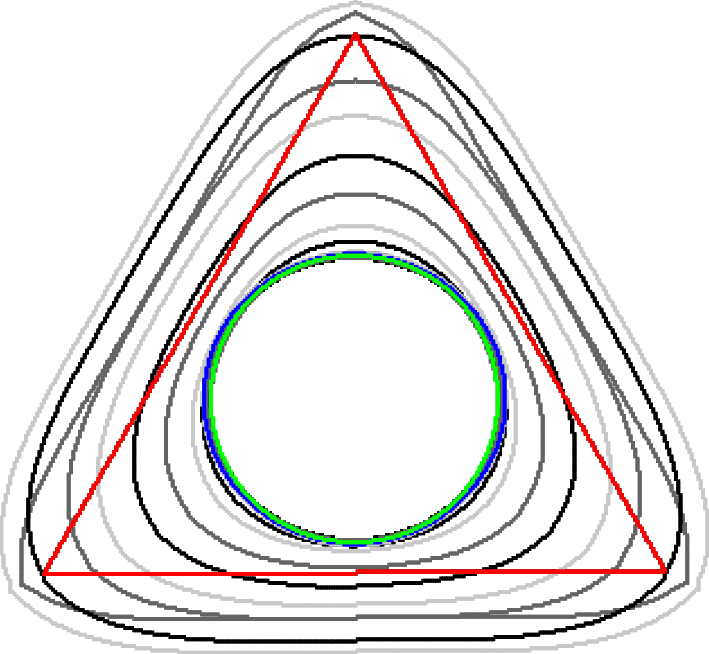
\includegraphics[scale=0.10]{figures/shape-flow/summaries-r8/triangle.png}

\vspace{1.5em}

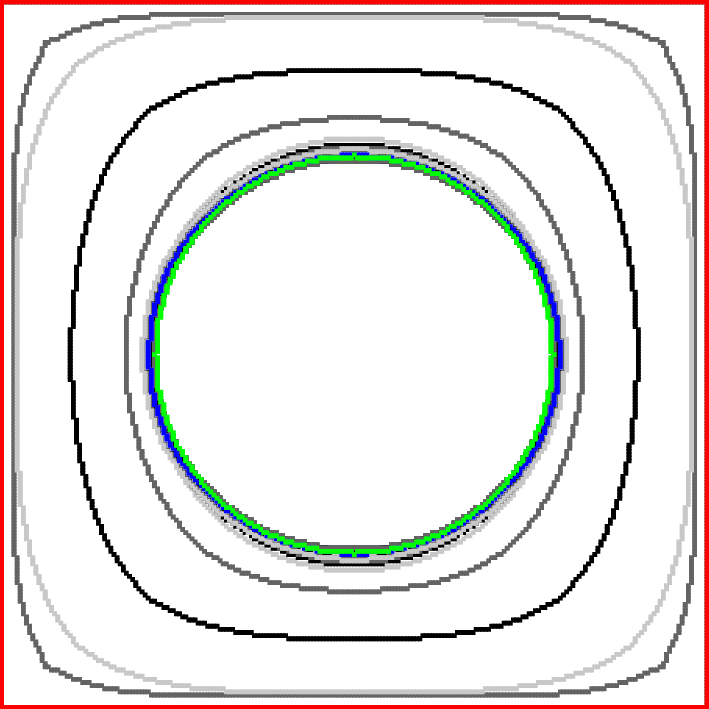
\includegraphics[scale=0.08]{figures/shape-flow/summaries-r8/square.png}

\vspace{1.5em}

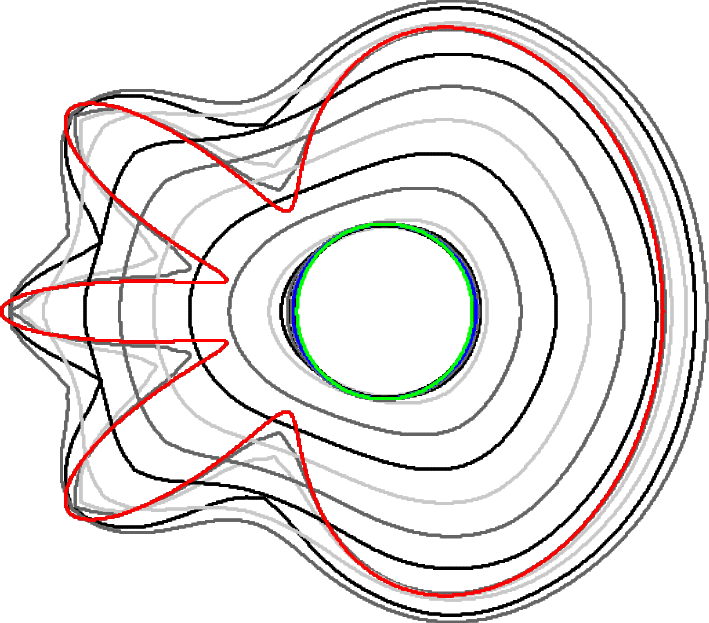
\includegraphics[scale=0.10]{figures/shape-flow/summaries-r8/flower.png}

\vspace{1.5em}

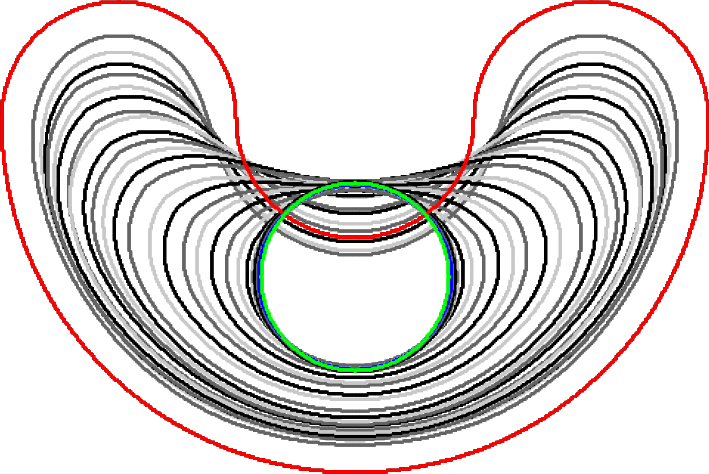
\includegraphics[scale=0.10]{figures/shape-flow/summaries-r8/bean.png}
\end{minipage}%
\begin{minipage}{0.75\textwidth}
\center
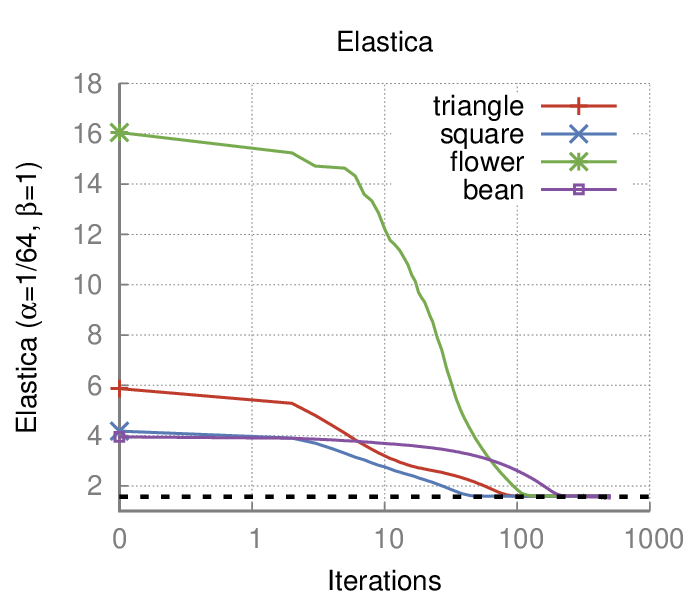
\includegraphics[scale=0.22]{figures/shape-flow/plots/elastica.png}

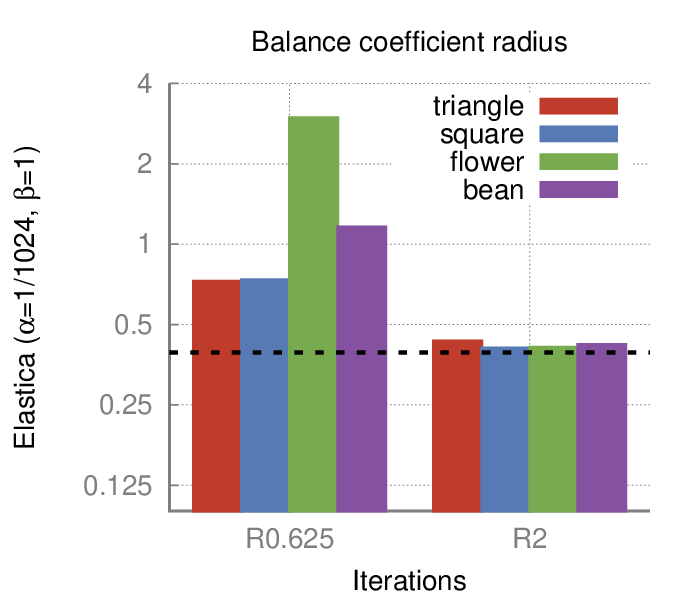
\includegraphics[scale=0.22]{figures/shape-flow/plots/bars.png}
\end{minipage}
    \caption{\textbf{GFA experiments}. In the left, the evolution of various shapes given by the GFA $(h=1/8,r=2)$, that is, the estimation disk has a radius of $16$ pixels. The red and blue contours highlight initial and final contours. The green contour is the optimum solution. The top right graph describes the reduction in elastica energy. The dotted line marks the optimum energy value (an Euclidean disk of radius $8$, or a disk digitization with $64$ pixels of radius with $h=1/8$). The bottom right graph points out the importance of a right choice of the balance coefficient radius.}
\label{fig:graph-flow-experiments}
\end{figure}

Remarkably, the GFA escapes premature local minima and even achieves the global optimum of the elastica energy for some cases. In~\cref{fig:graph-flow-expand} we show the results of elastica minimization for $\vec{\Theta} = ( r=2,h=1/8,\alpha=1/1024,\beta=1 )$. The GFA correctly expands the shapes to the optimum disk of radius $32$. However, we may have a premature interruption of the evolution if a small estimation disk radius is chosen, as illustrated in the bottom right graph of~\cref{fig:graph-flow-experiments}.
%
%
\begin{figure}
\center
\subfloat[]{
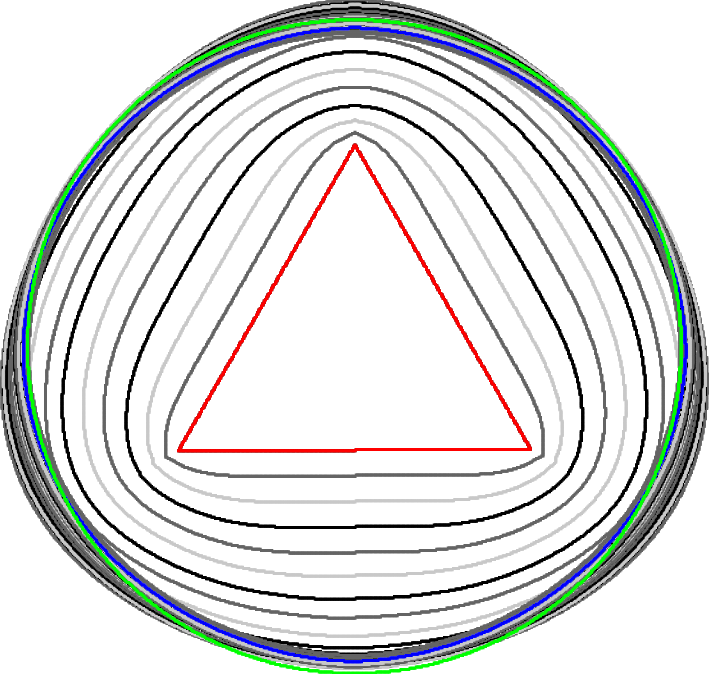
\includegraphics[scale=0.13]{figures/shape-flow/summaries-r32/triangle.png}}\hspace{1.5em}%
\subfloat[]{
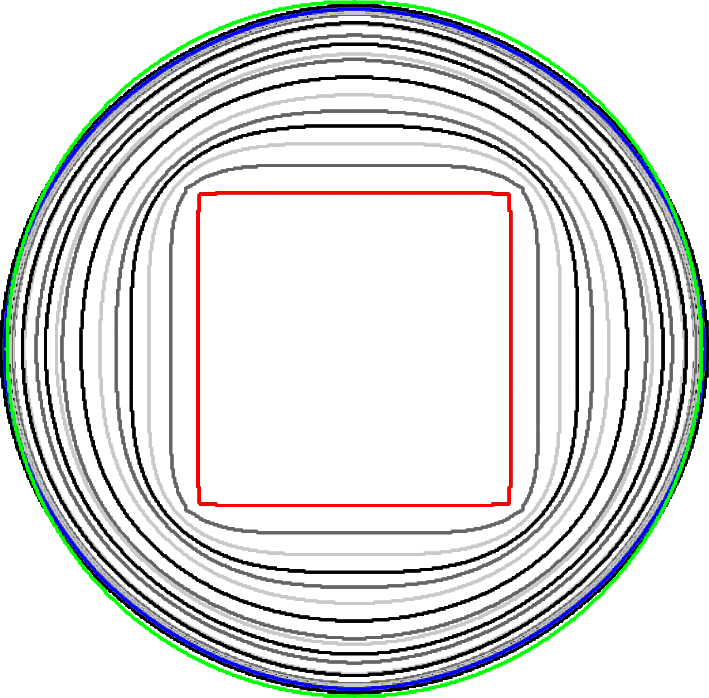
\includegraphics[scale=0.13]{figures/shape-flow/summaries-r32/square.png}}\hspace{1.5em}%
\subfloat[]{
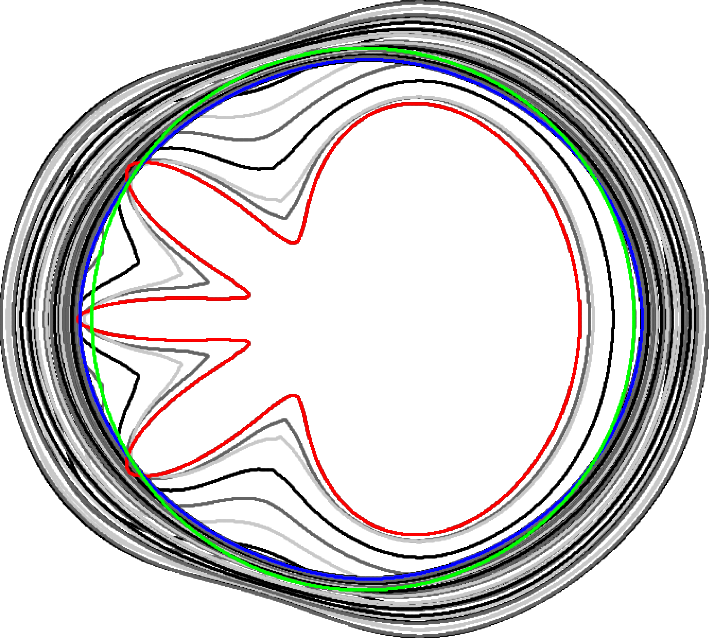
\includegraphics[scale=0.15]{figures/shape-flow/summaries-r32/flower.png}}
\caption{\textbf{GFA can expand the initial shape}. Shapes evolutions by GFA with $\vec{\Theta}(h=1/8,r=2,\alpha=1/1024, \beta=1)$ as the elastica estimator parameters. The green contour highlights the optimum shape.}
\label{fig:graph-flow-expand}
\end{figure}
%
%
The computations can be done in parallel for each member of the neighborhood of shapes. \Cref{tab:summary-graph-flow-running-time} shows the running times where the candidate graphs are evaluated in parallel. These times can be further improved by parallelizing the computation of the balance coefficient as well as the elastica estimator evaluation.
%
%
\begin{figure}[h!]
\center
\captionsetup{type=table}
\footnotesize
	\caption{\textbf{Running time of GFA}. The GFA achieves running times lower than one second per iteration when the shape neighbors are evaluated separately (executed in a Intel Corei7 $1.8GHz$ processor with $16gb$ of ram). These running times could be further improved, for instance by parallelization of balance coefficient  or elastica energy computations.}\label{tab:summary-graph-flow-running-time} 
\begin{tabular}{|l|c|c|c|c|}
\hline
& Pixels & It & Time & Time/It\\
\hline
Triangle & 33256 & 120 & 49.6s & 0.4s \\
Square & 51259 & 60 & 24.6s & 0.4s \\
Flower & 119789 & 150 & 132.8s & 0.9s \\
Bean & 100504 & 300 & 148.4s & 0.5s \\
\hline
\end{tabular}
\end{figure}
%
%
Finally, the GFA is easily modifiable to accomodate image terms, which makes it suitable for image processing tasks. Next, we are going to explore some of these possibilitites in image segmentation.
%
%

\section{Applications in image processing}

In this section, we explore the potential of the GFA in image segmentation tasks. The GFA can indeed be extended to include a data fidelity term.
We present the results of two experiments. The first one is a supervised segmentation and the second one is an unsupervised segmentation. For images, since the digitization process cannot be done with an arbitrary resolution, we set $h=1$ in all experiments. The experiments were executed on an Intel Corei7 $1.8GHz$ processor with $16gb$ of RAM.


\subsection{Supervised segmentation}

The goal of this experiment is to illustrate the regularization properties of the GFA and to highlight the role of the data term in our approach. The data term employed in this experiment is the same used by Boykov-Jolly in their classical graph cut model~\cite{boykov01graphcut}. 

\subsubsection{Data term}
We update the graph construction described in~\cref{sec:graph-cut-model} to accomodate the data term. In particular, we define two new sets of vertices $\mathcal{V}_{fg}$ and $\mathcal{V}_{bg}$ as the set of foreground and background seeds, respectively. Those are given as input.

Let $\vec{x} \in \{0,1\}^{|S|}$ represent the label of each pixel in the image ($0$ for background and $1$ for foreground). We define the data term as
%
%
\begin{align*}
    data(S,\gamma_r,\gamma_b) &= \gamma_r \sum_{P \in S}{ \psi(x_P) } + \gamma_b \sum_{P \in S}\sum_{Q \in \mathcal{N}_{4}(P)}{\phi_{(P,Q)}},
\end{align*}
where $\gamma_r \geq 0$ and $\gamma_b \geq 0$ are parameters controlling the influence of the regional and boundary terms, respectively. Given the image $I:\Omega \rightarrow [0,1]^3$, the unary and pairwise terms are defined as
\begin{align*}
	\psi(x_P) &= \left\{ \begin{array}{ll}
	-\ln  H_{bg}\big( I(P) \big), & \text{if } x_P=0  \\[1em]	
	-\ln  H_{fg}\big( I(P) \big), & \text{if } x_P=1,
	\end{array}\right.\\[1em]
	\phi_{(P,Q)} &= \left\{ \begin{array}{ll}
	\displaystyle \exp{ \left(- \frac{(I(P) - I(Q))^2}{|P-Q|} \right) }, & Q \in \mathcal{N}_4(P) \\[1em]
	0, & \text{otherwise}.
	\end{array}\right.
\end{align*}
%
%
The terms $H_{bg}$ and $H_{fg}$ are mixed Gaussian distribution constructed from the foreground and background seeds. The updated capacity function is described in~\cref{tab:updated-capacity-function}.
%
%
\begin{table}
\setlength{\extrarowheight}{0.75em}
\begin{center}
\footnotesize
	\caption{\textbf{Updated capacity function.} The capacity function of~\cref{tab:edge-capacity} is updated to accommodate the data term. The constant $M$ is simply the maximum of all capacities, i.e. $M = \max_{e \in \mathcal{E} }{ c(e) }$.}\label{tab:updated-capacity-function}
\begin{tabular}{|c|c|c|}
\hline
\textbf{edge} $e$ & $\mathbf{c(e)}$ & \textbf{for}\\
\hline
$\{v_P, v_Q\}$ & $\beta \cdot \big(u_r(S,P) + u_r(S,Q)\big) + \gamma_b \cdot \phi_{(P,Q)}$ & $\{v_P,v_Q\} \in \mathcal{E}_{u}$\\
\hline
\multirow{3}{*}{$\{s,v_P\}$} & $\gamma_r \cdot \psi(0)$ & $P \in O_n(S), v_P \notin \mathcal{V}_{fg} \cup \mathcal{V}_{bg}$\\
& $M$ & $v_P \in \mathcal{V}_{s} \cup \mathcal{V}_{fg}$ \\
\hline
\multirow{3}{*}{$\{v_P, t\}$} & $\gamma_r \cdot \psi(1)$ & $P \in O_n(S), v_P \notin \mathcal{V}_{fg} \cup \mathcal{V}_{bg}$ \\
& $M$ & $v_P \in \mathcal{V}_{t} \cup \mathcal{V}_{bg}$  \\
\hline
\end{tabular}
\end{center}
%% where the constant $M$ is defined such that
%% \begin{align*}
%% M &= \max_{e \in \mathcal{E} }{ c(e) }.
%% \end{align*}
\end{table}
%
%
To handle bias due to the magnitude difference between data and geometry terms, we normalize them in groups. Regional and boundary terms $\psi,\phi$ are normalized to the interval $[0,1]$ with respect to their values. The same is done, separately, for the curvature term.

To minimize parameter dependence from the image input, we also apply a parameter normalization. Given parameters $\alpha, \gamma_b, \gamma_r$ and an initial segmentation $I_0$ (which is necessary to start segmentation by GFA), consider the corresponding normalized parameters:
%
%
\begin{align*}
    \alpha' & = \alpha \times 4\pi^2/Per^2(I_0) \\
	\gamma_r' & = \gamma_r \times \hat{E}(I_0)/data(I_0,\gamma_r,\gamma_b) \\	
	\gamma_b' & = \gamma_b \times \hat{E}(I_0)/data(I_0,\gamma_r,\gamma_b)		
\end{align*}

Given that segmentation with GFA was started with parameters $\alpha=\gamma_r=\gamma_b=1$, 
the normalized parameters set the disk of perimeter $Per(I_0)$ as the optimum shape 
for the elastica energy and make the data contribution from $I_0$ to have the same
value as the elastica energy computed for the initial segmentation and unormalized
parameters.
%
%
\subsubsection{Experiments}
We need an initial contour to start the GFA. The initial contour is given by the grabcut algorithm~\cite{rother04grabcut}, a variant of classical graph cut segmentation~\cite{boykov01graphcut} which is implemented in the OpenCV library.

For this experiment, we used a selection of $212$ images of the Validation 2017 subset of the Coco dataset~\cite{lin2014microsoft}. The Coco dataset comprises over $328$k images spreaded over $91$ categories and $11$ super-categories. \Cref{tab:image-categories-distribution} summarizes the quantity of selected images per super-category. 
%
%
\begin{table}
\footnotesize
	\caption{\textbf{Distribution of selected images.} The quantity of selected images per Coco super-category. A total of $212$ images were selected.}\label{tab:image-categories-distribution}
\begin{tabular}{cccccc}
\textbf{Person} & \textbf{Vehicle} & \textbf{Food} & \textbf{Animal} & \textbf{Outdoor Obj.} & \textbf{Sports} \\
24 & 22 & 22 & 34 & 16 & 19 \\[1em]
\textbf{Kitchenware} & \textbf{Furniture} & \textbf{Appliance} & \textbf{Electronics} & \textbf{Indoor Obj.} & \\
19 & 17 & 9 & 10 & 19 &
\end{tabular}
\end{table}
%
%
The following experiment studies the influence of inserting the data term into the graphcut formulation. It consists in the following steps:
\begin{enumerate}
\item manual selection of foreground and background seeds for each selected image;
\item computation of the grabcut segmentation;
\item and then using the grabcut segmentation as input for two versions of the GFA: one with the data term described in the previous section and another without.
\end{enumerate}

In~\cref{fig:coco-experiment-sample} we show a sample of the images
used in the experiment. All the results are available online at the paper's
website.

\cref{tab:coco-experiment-parameter} lists the GFA parameters used for this experiment.
%
%
\begin{table}
\center
\footnotesize
	\caption{\textbf{Supervised experiment parameters}. List of the GFA parameters for the supervised segmentation experiment.}\label{tab:coco-experiment-parameter}
\begin{tabular}{cccc}
\textbf{Estimation radius} & \textbf{Opt. band width} & \textbf{Neighborhood size} & \textbf{Iterations} \\
$\mathbf{(r)}$ & $\mathbf{(n)}$ & $\mathbf{(k)}$ & \textbf{(maxit)}\\
5 & 4 & 3 & 20\\[1em]
\textbf{Length weight} & \textbf{Curvature weight} & \textbf{Boundary weight} & \textbf{Region weight}\\
$\boldsymbol{(\alpha)}$ & $\boldsymbol{(\beta)}$ & $\boldsymbol{(\gamma_b)}$ & $\boldsymbol{(\gamma_r)}$\\
10 & 1 & 1 & 1
\end{tabular}
\end{table}
%
%
\begin{table}
\footnotesize
	\caption{\textbf{Supervised experiment running times}. The average time per iteration is of $0.7$s.}\label{tab:coco-experiment-running-time}
\center
\begin{tabular}{cccc}
\textbf{Highest} & \textbf{Lowest} & \textbf{Average} & \textbf{Average per iteration} \\
50.3s & 3.3 & 15.1s & 0.7s\\
\end{tabular}
\end{table}
%
%
\begin{figure}
\center
\subfloat[Coco annotations for kite, moto and giraffe]{
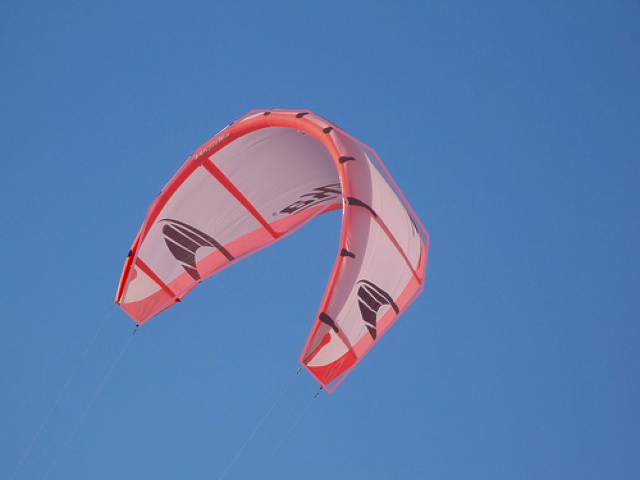
\includegraphics[scale=0.2]{figures/coco-experiment/sample-images/kite/coco-annotation.png}\hspace{1em}
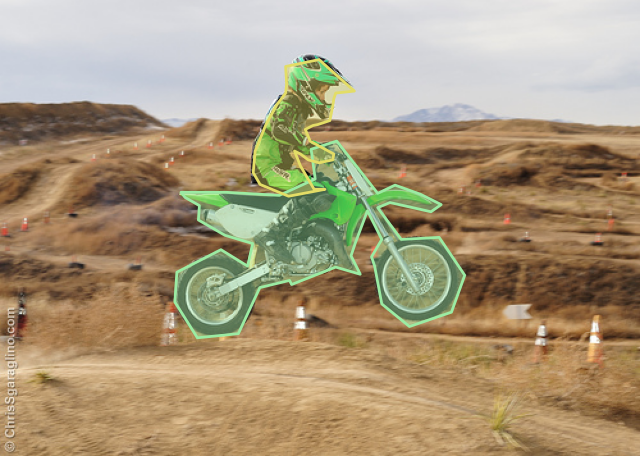
\includegraphics[scale=0.2]{figures/coco-experiment/sample-images/moto/coco-annotation.png}
\hspace{1em}
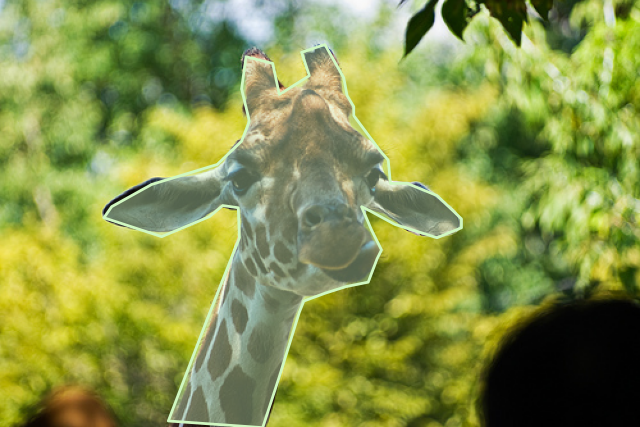
\includegraphics[scale=0.2]{figures/coco-experiment/sample-images/giraffe/coco-annotation.png}
}%

\subfloat[Grabcut segmentation]{
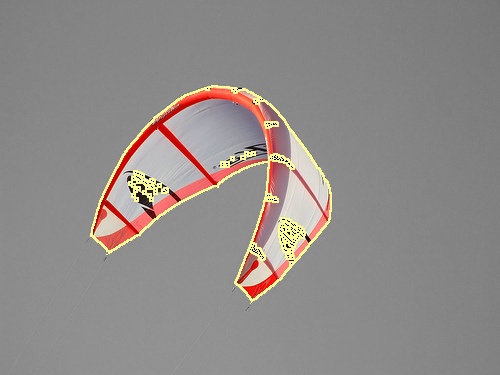
\includegraphics[scale=0.2]{figures/coco-experiment/sample-images/kite/gc-seg.png}
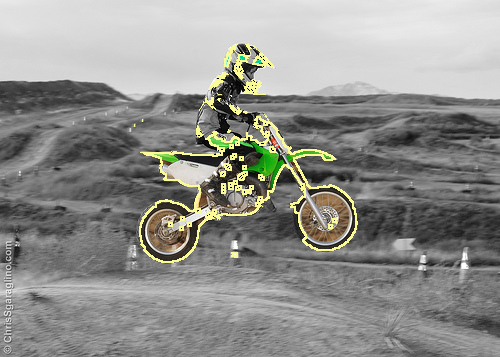
\includegraphics[scale=0.2]{figures/coco-experiment/sample-images/moto/gc-seg.png}
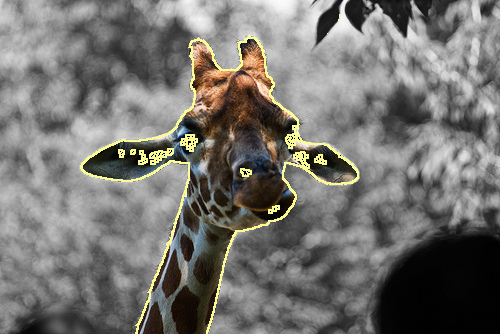
\includegraphics[scale=0.2]{figures/coco-experiment/sample-images/giraffe/gc-seg.png}
}

\subfloat[GFA without data term]{
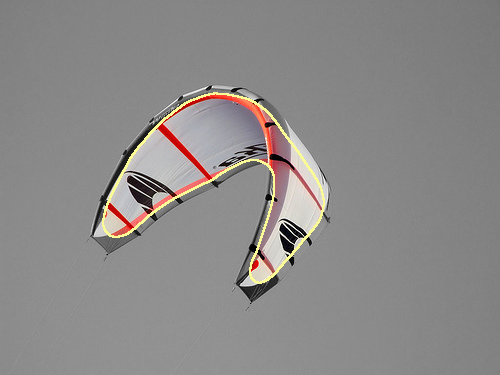
\includegraphics[scale=0.2]{figures/coco-experiment/sample-images/kite/corrected-seg-without-data.png}
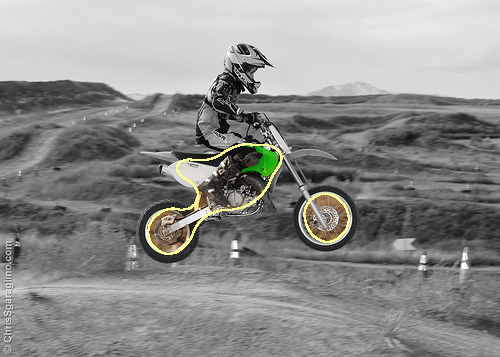
\includegraphics[scale=0.2]{figures/coco-experiment/sample-images/moto/corrected-seg-without-data.png}
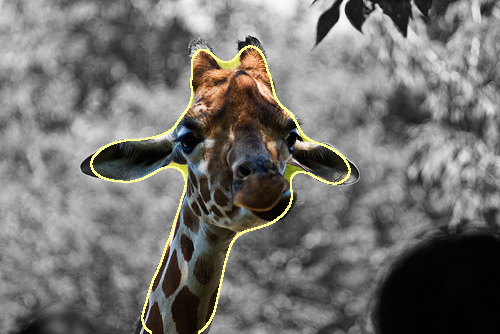
\includegraphics[scale=0.2]{figures/coco-experiment/sample-images/giraffe/corrected-seg-without-data.png}
}

\subfloat[GFA with data term]{
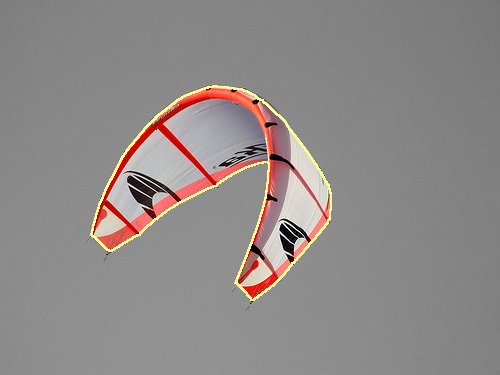
\includegraphics[scale=0.2]{figures/coco-experiment/sample-images/kite/corrected-seg-with-data.png}
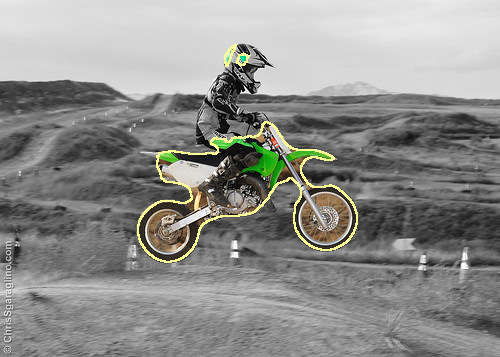
\includegraphics[scale=0.2]{figures/coco-experiment/sample-images/moto/corrected-seg-with-data.png}
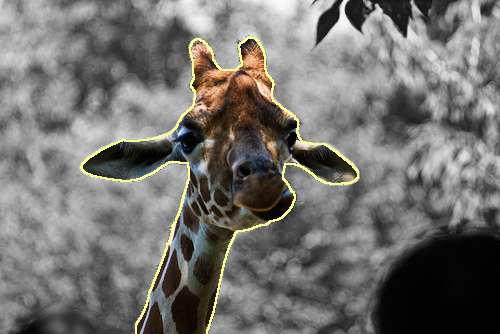
\includegraphics[scale=0.2]{figures/coco-experiment/sample-images/giraffe/corrected-seg-with-data.png}
}
\caption{\textbf{Some results of the supervised segmentation experiment}. Coco annotations are shown in the first line. In the next rows we present the same image segmented by grabcut and corrected by the GFA without and with data term.  }
\label{fig:coco-experiment-sample}
\end{figure}
%
%
The first observation is that the GFA regularizes the initial grabcut segmentation contour with respect to the elastica energy. In~\cref{fig:coco-tangent-profile} we display the tangent profile of both grabcut segmentation and the one corrected by the GFA. We clearly observe the regularization effect of the GFA with respect to the grabcut profile. The value of the elastica energy of the contour and its number of inflection points is also greatly reduced, as summed up in~\cref{fig:coco-summary-regularization}.

The second observation is that the data term has an important role in the quality of the segmentation with respect to precision and recall metrics. This is shown in the box plot of~\cref{fig:coco-summary-precision-recall}. That means that a contour evolution model with no data term, such as threshold dynamics, is insufficient to recover segmentations of good quality. In fact, executing the GFA without data term will eventually transform the contour in one or more circles, and we can have an arbitrary bad value for the recall. We can see some of these undesirable effects in the third line of~\cref{fig:coco-experiment-sample}: the kite area is overly reduced; the motorcycle is separated in two disconnected components; and the giraffe loses parts of its ears.

The third observation is that the GFA indeed presents the completion effect, which was expected from regularization by the elastica energy. This property is particularly useful for the segmentation of thin and elongated objects, but not only. It also helps to remove oversegmented components which are particularly common in graph cut based models. In~\cref{fig:coco-completion} we give some examples of contour completion.

Finally, we remark that all image segmentations were executed using the same set of parameters. That is not ideal. Low resolution images should be segmented using a smaller estimation radius, for example. Therefore, all the results presented here could be eventually improved by tuning the parameters accordingly. An example of this is given in~\cref{fig:coco-parameter-tuning}.

A summary of the running time is presented in~\cref{tab:coco-experiment-running-time}. The average running time per iteration is of $0.7$s. We remark that in several cases we need fewer than $5$ iterations to greatly improve the regularization metrics such as elastica and inflection points. However, to recover the completion effect we may need more iterations.
%
%
\begin{figure}
\center
\subfloat[Grabcut segmentation (left) and corrected segmentation by GFA (right).]{
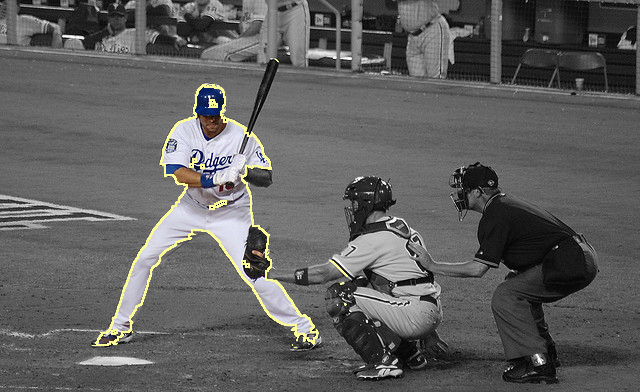
\includegraphics[scale=0.25]{figures/coco-experiment/tangent-profile/baseball/gc-seg.png}\hspace{1em}
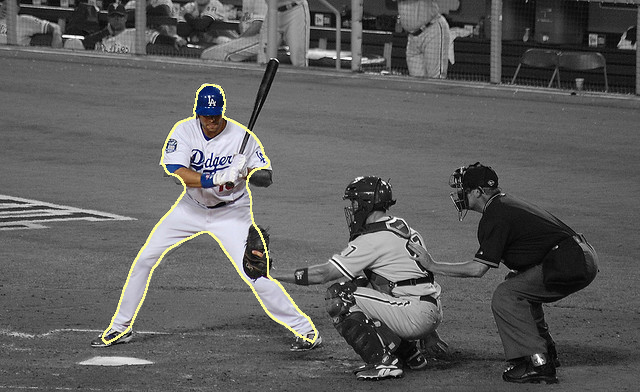
\includegraphics[scale=0.25]{figures/coco-experiment/tangent-profile/baseball/corrected-seg-with-data.png}
}

\subfloat[Tangent profile for grabcut (left) and GFA (right) segmentations.]{
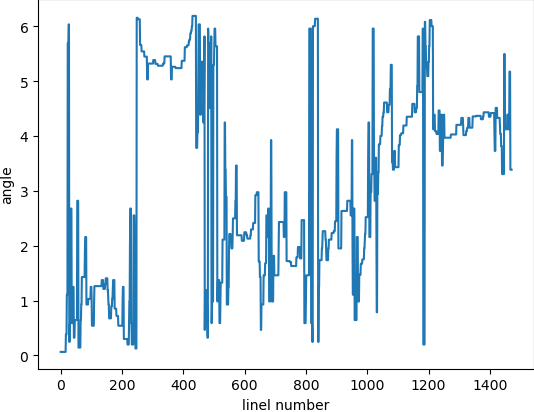
\includegraphics[scale=0.42]{figures/coco-experiment/tangent-profile/baseball/tangent-profile-gc.png}\hspace{1em}
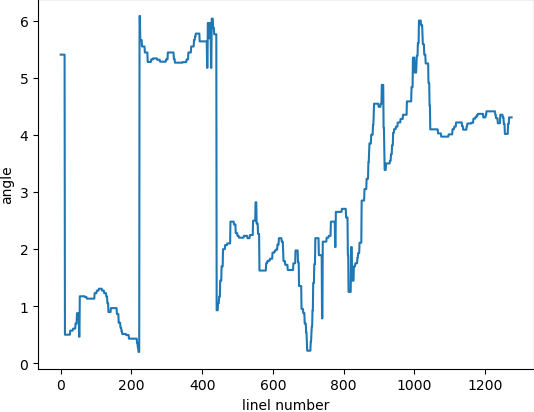
\includegraphics[scale=0.42]{figures/coco-experiment/tangent-profile/baseball/tangent-profile-cc.png}
}
\caption{\textbf{Contour regularization.} The GFA normalizes the contour with respect to the elastica energy. This is illustrated by the tangent profile of the grabcut segmentation and the one corrected by GFA.}
\label{fig:coco-tangent-profile}
\end{figure}
%
%
\begin{figure}
\center
\subfloat[Recall and precision results with respect to Coco annotations.\label{fig:coco-summary-precision-recall} ]{
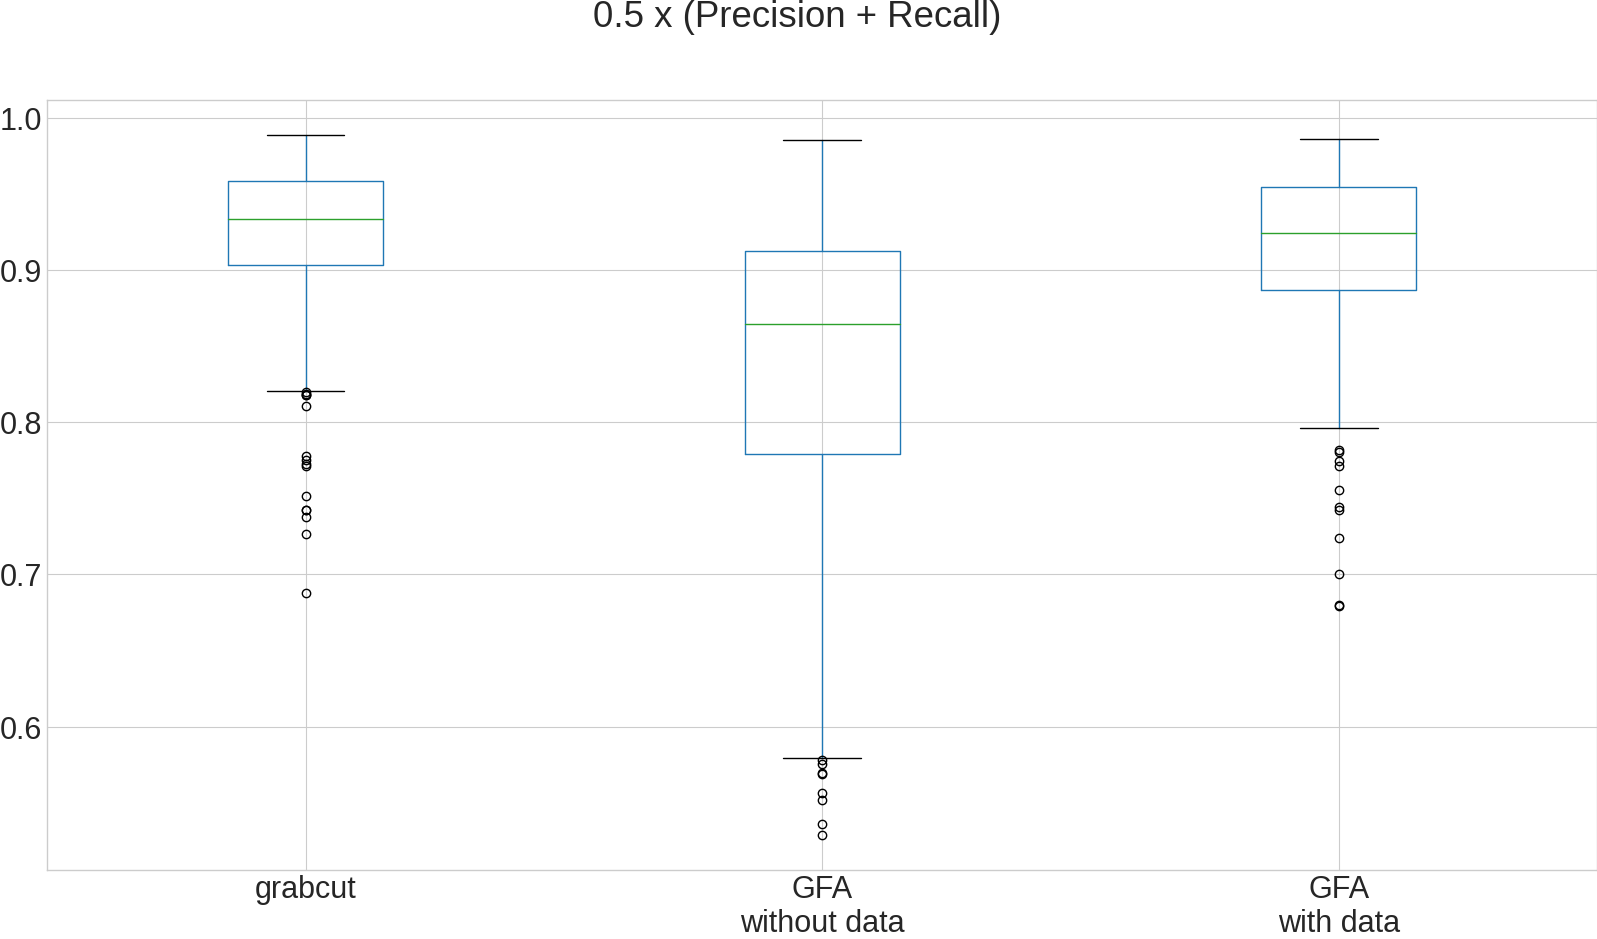
\includegraphics[scale=0.25]{figures/coco-experiment/box-plot-mixed.png}
}

\subfloat[Contour regularization metrics for GFA with respect grabcut.\label{fig:coco-summary-regularization}]{
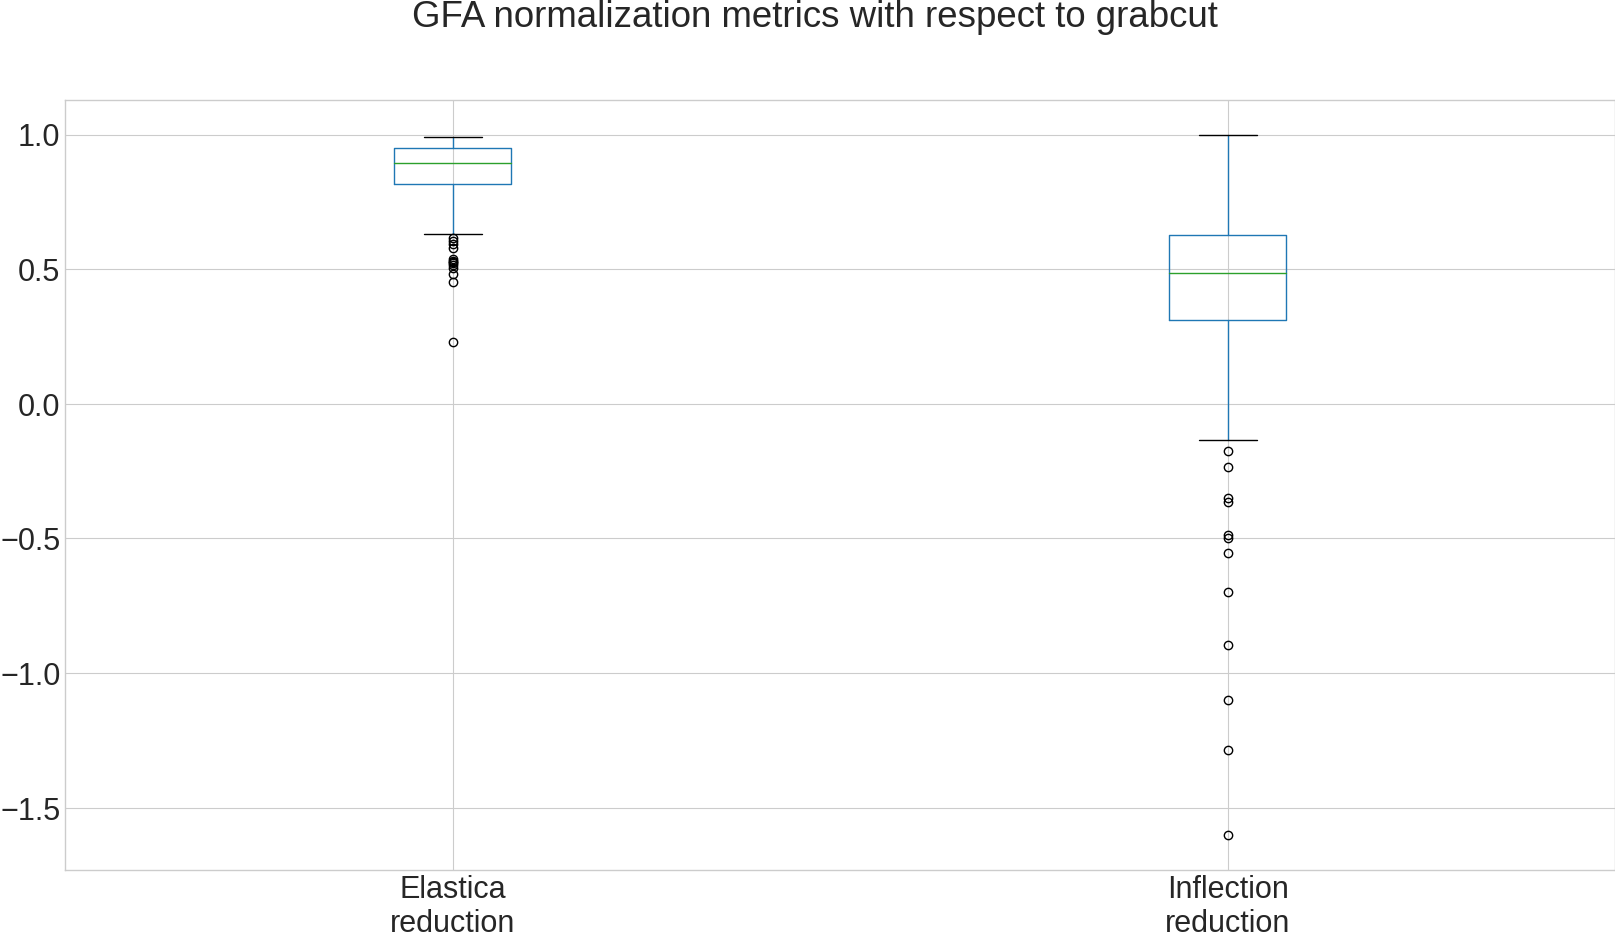
\includegraphics[scale=0.25]{figures/coco-experiment/box-plot-correction.png}
}

\caption{\textbf{Summary statistics.} The GFA give results as good as grabcut with respect to precision and recall, but with a much simpler and easy to describe (and to store) contour.}
\end{figure}
%
%
\begin{figure}
\center
\subfloat[Using $r=5$ ($(P+R)/2=0.78$)]{
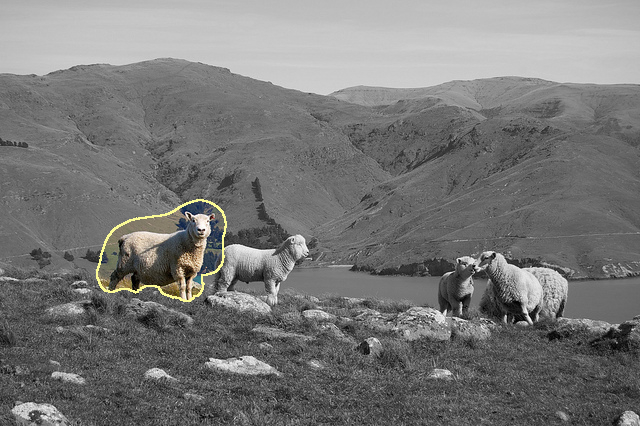
\includegraphics[scale=0.25]{figures/coco-experiment/parameter-tuning/sheep_r5/corrected-seg-with-data.png}}\hspace{1em}
\subfloat[Using $r=3$ ($(P+R)/2=0.94$)]{
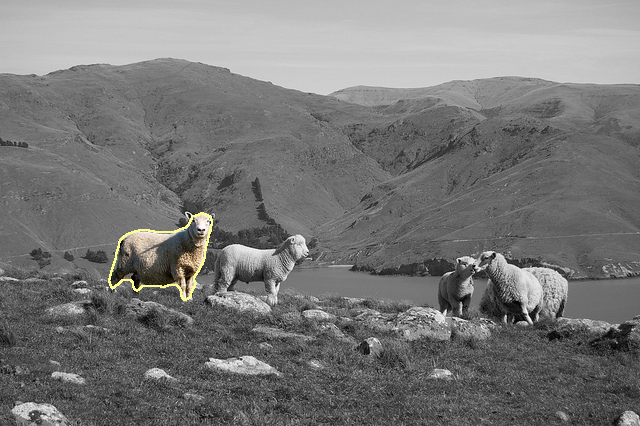
\includegraphics[scale=0.25]{figures/coco-experiment/parameter-tuning/sheep_r3/corrected-seg-with-data.png}}
\caption{\textbf{Parameter tuning.} The GFA was executed with the same set of parameters for all images, but we can recover better results by tuning the parameter for each image separately. In this example, the low scale of the image asks for a lower estimation radius. The precision plus recall average goes from $0.78$ to $0.94$ by using a radius of $3$ instead of $5$. }
\label{fig:coco-parameter-tuning}
\end{figure}
%
%
\subsection{Unsupervised binary segmentation}
The goal of this experiment is to illustrate the flexibility of the GFA with respect to the data fidelity term. In this experiment, we employed a Chan-Vese alike data term~\cite{chan01}, i.e., we penalize the square mean error between pixel intensity and the average foreground color (similarly for the background). We define the initial solution as an uniform collection of disks covering the image domain.

In this application, our strategy to avoid local minima is slightly different. We use a neighborhood of shapes composed by random perturbations of the initial contour and we allow evolution if and only if the previous energy value is reduced. This strategy leads to higher running times, but since the digital components are treated independently, we believe that running times can be greatly reduced by implementing a more agressive parallelization strategy, for example, using GPUs. 

The algorithm can evolve the contours in favor of contour completion or breaking them according to the relative weights given for the elastica and data terms. We show the results of some experiments in~\cref{fig:GF-chan-vese-alike}.

\begin{figure}
\center
\subfloat[Segmentation by grabcut]{
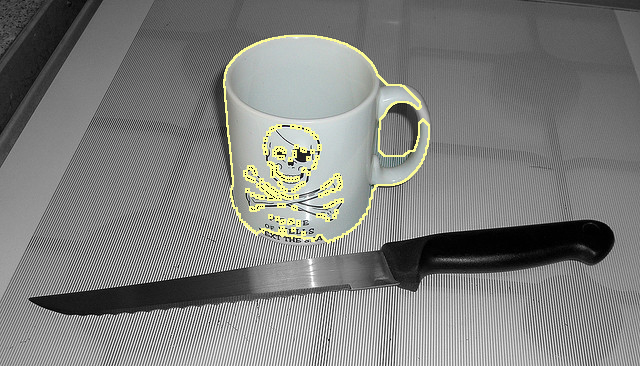
\includegraphics[scale=0.15]{figures/coco-experiment/completion/cup/gc-seg.png}\hspace{0.125em}
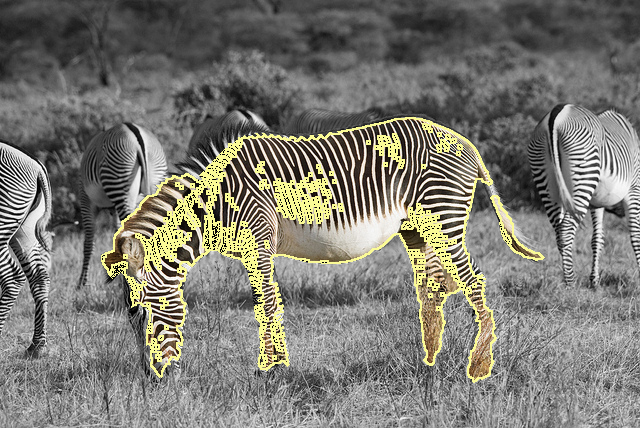
\includegraphics[scale=0.13]{figures/coco-experiment/completion/zebra/gc-seg.png}
\hspace{0.125em}
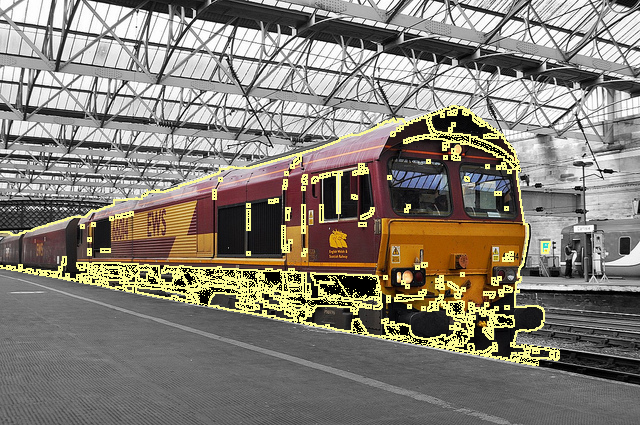
\includegraphics[scale=0.13]{figures/coco-experiment/completion/train/gc-seg.png}\hspace{0.125em}
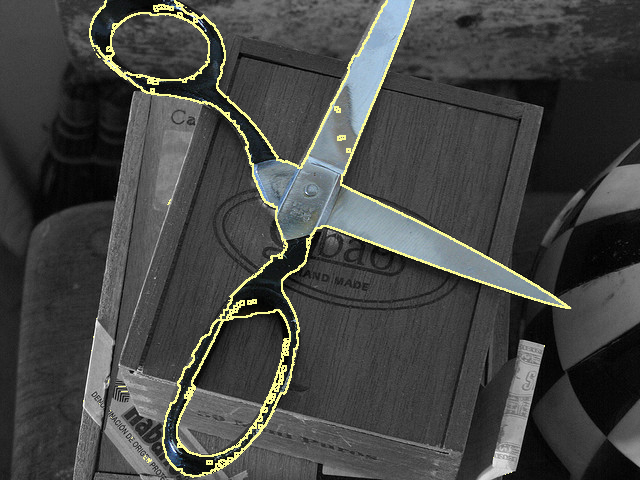
\includegraphics[scale=0.12]{figures/coco-experiment/completion/scissors/gc-seg.png}
}%

\subfloat[Segmentation corrected by GFA]{
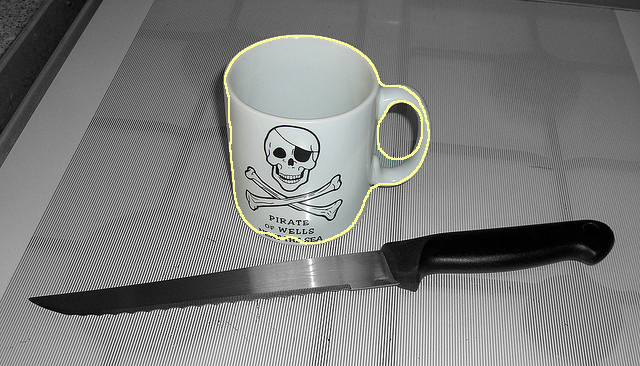
\includegraphics[scale=0.15]{figures/coco-experiment/completion/cup/corrected-seg-with-data.png}\hspace{0.125em}
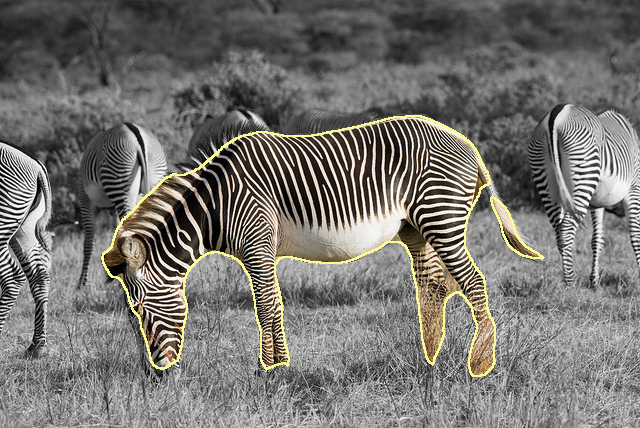
\includegraphics[scale=0.13]{figures/coco-experiment/completion/zebra/corrected-seg-with-data.png}
\hspace{0.125em}
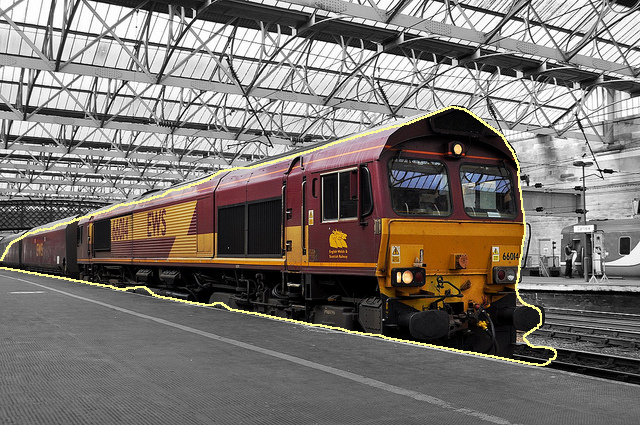
\includegraphics[scale=0.13]{figures/coco-experiment/completion/train/corrected-seg-with-data.png}\hspace{0.125em}
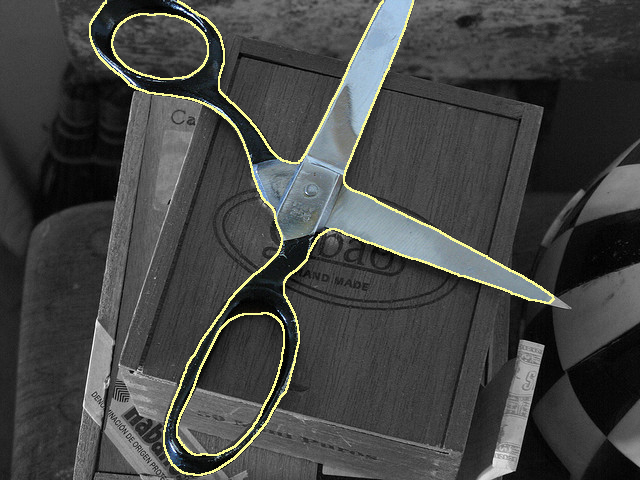
\includegraphics[scale=0.12]{figures/coco-experiment/completion/scissors/corrected-seg-with-data.png}
}%
\caption{\textbf{Contour completion.} The GFA favors connected components due to the completion effect of the elastica energy. That is particularly useful to avoid oversegmentation artefacts.}
\label{fig:coco-completion}
\end{figure}

\begin{figure}
\center
\subfloat[$22$ iterations ($52$s).]{
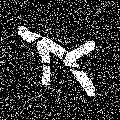
\includegraphics[scale=0.5]{figures/chan-vese-alike/branch/branch-noisy.png}
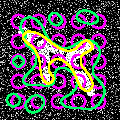
\includegraphics[scale=0.5]{figures/chan-vese-alike/branch/contours.png}
}\hspace{1em}%
\subfloat[$26$ iterations ($76$s).]{
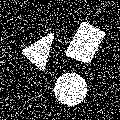
\includegraphics[scale=0.5]{figures/chan-vese-alike/simple-geometry/simple-geometry-noisy.png}
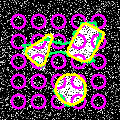
\includegraphics[scale=0.5]{figures/chan-vese-alike/simple-geometry/contours.png}
}%
\caption{\textbf{Chan-Vese alike data term.} The initial contour is highlighted in pink and the final contour in yellow. An intermediate contour is also highlighted in green. A proper parameter setting favors component completion (left) or component break (right). Images are $100\times100$. }
\label{fig:GF-chan-vese-alike}
\end{figure}
%
%
%
%
\section{Conclusion}
%
%
We presented a discrete shape evolution algorithm driven by the elastica energy. The GFA is built on recent results on the multigrid convergence of curvature and tangent estimators and its main step consists in computing the minimum cut of candidate graphs. A candidate graph is constructed for each element in a neighborhood of shapes of the current digital set and its minimum cut gives a candidate shape. At each iteration, the GFA selects the candidate shape with lowest elastica energy. We have shown that our model can escape local energy minima during the shape evolution by using a very simple neighborhood of shapes. Indeed, our experiments converged to the shape of minimum elastica energy. 

Next, we presented some applications in image processing. The GFA produces contours with fewer inflection points, smoother tangent profiles and lower elastica energy than those produced from grabcut. That is done while keeping high values of precision and recall with respect to the Coco annotated images used in our experiments. Finally, we presented an unsupervised segmentation model based on the classical Chan-Vese data term, which demonstrates the flexibility of the model. 

One of the strengths of our model is that the curvature estimation is based on digital data solely and it is not attached to a curve model, which may restrict the curve evolution and pose technical difficulties regarding its update. Secondly, the GFA is highly parallelizable. We believe that a GPU implementation will greatly reduce the running times of our algorithm for all presented applications. The bottleneck is in the minimum cut computation, as it is difficult to come up with a parallel implementation, but since the latter is computed along a thin band of the shape contour, we believe that this is a minor problem.

There are some possible paths for future work. Firstly, the graph construction part of the algorithm can be optimized. In the current version, the graph is constructed at every iteration, but most of the time, the graph structure changes very slightly and this can be used to optimize its construction. Secondly, we use a very simple neighborhood of shapes in the supervised segmentation problem, i.e., based on dilations and erosions of the initial shape. The contour completion property of the model could be enhanced by employing different neighborhoods. For example, we could elongate the initial shapes in regions of high curvature to obtain a stretched neighborhood of shapes. This could be particularly useful in the segmentation of thin and elongated objects such as blood vessels.
%
%
%
%
\bibliographystyle{siamplain}
\bibliography{gf-paper}

\end{document}

